\chapter{BaseLib Level 3}
\chaptermark{Level 3}


BaseLib Level 3 deals about the problem of configuration that is really similar to serialization in Object Oriented Programming (OOP) in BaseLib. The basic issue addressed here is the reding and writing of a configuration file from a file or generally from a stream, the stream is a formatted document where it is saved a configuration of the system, a configuration must also be thinked as a backed up set of instances of all the classes in a particular life moment of the system (OOP serialization). \\


The main tool that lets the user select which class to load and setting the parameters is the \textit{Configuration Database}, a \textit{Configuration Database}, that was just partially covered in the previous chapters, is a tree data structure that reflect the content of a configuration file (or stream). Using this philosopy every component of the framework that need configuration parameters must ask to this central entity that address configuration issues. \\


The whole BaseLib Level 3 could be divided in the following sections:
\begin{itemize}
 \item CDB
 \item other CDBs (stream oriented CDBs)
 \item Parser
\end{itemize}

The fundamental component of this level is the CDB, i.e. an implementation of a \texttt{Configuration Database} interface in \textit{/level1}. A CDB addresses the problem of which classes and which paramenters loading during the framework startup and reflect the system status (i.e. instantiated classes and attributes value) not only at the initialization but also during runtime; i.e. implements serialization.

Objects type registration and object instantiation is done by the previously analized GODB and ORDB; configuration database loading is the last step for the system inizialization. \\


The flow chart in Figure \ref{f:level3:objects} shows the order in which the logical components that compose the objects infrastructure, i.e. type registration, instantiation and serialization; are loaded by the BaseLib framework at application startup.

Loading an application that runs under the BaseLib framework lets the code first execute the compile time C++ code that create static and globally defined classes; part of this classes create the ORDB. Then a configuration file (or a stream) will be read and a configuration tree will be created, i.e. a CDB. When the ORDB and the CDB are ready a GODB is then filled up using the configuration of a CDB loading objects registered in the ORDB. This is the whole story; we try to better explain all this stuff with an example in the following. \\

\begin{figure}[h!]
 \begin{center}
  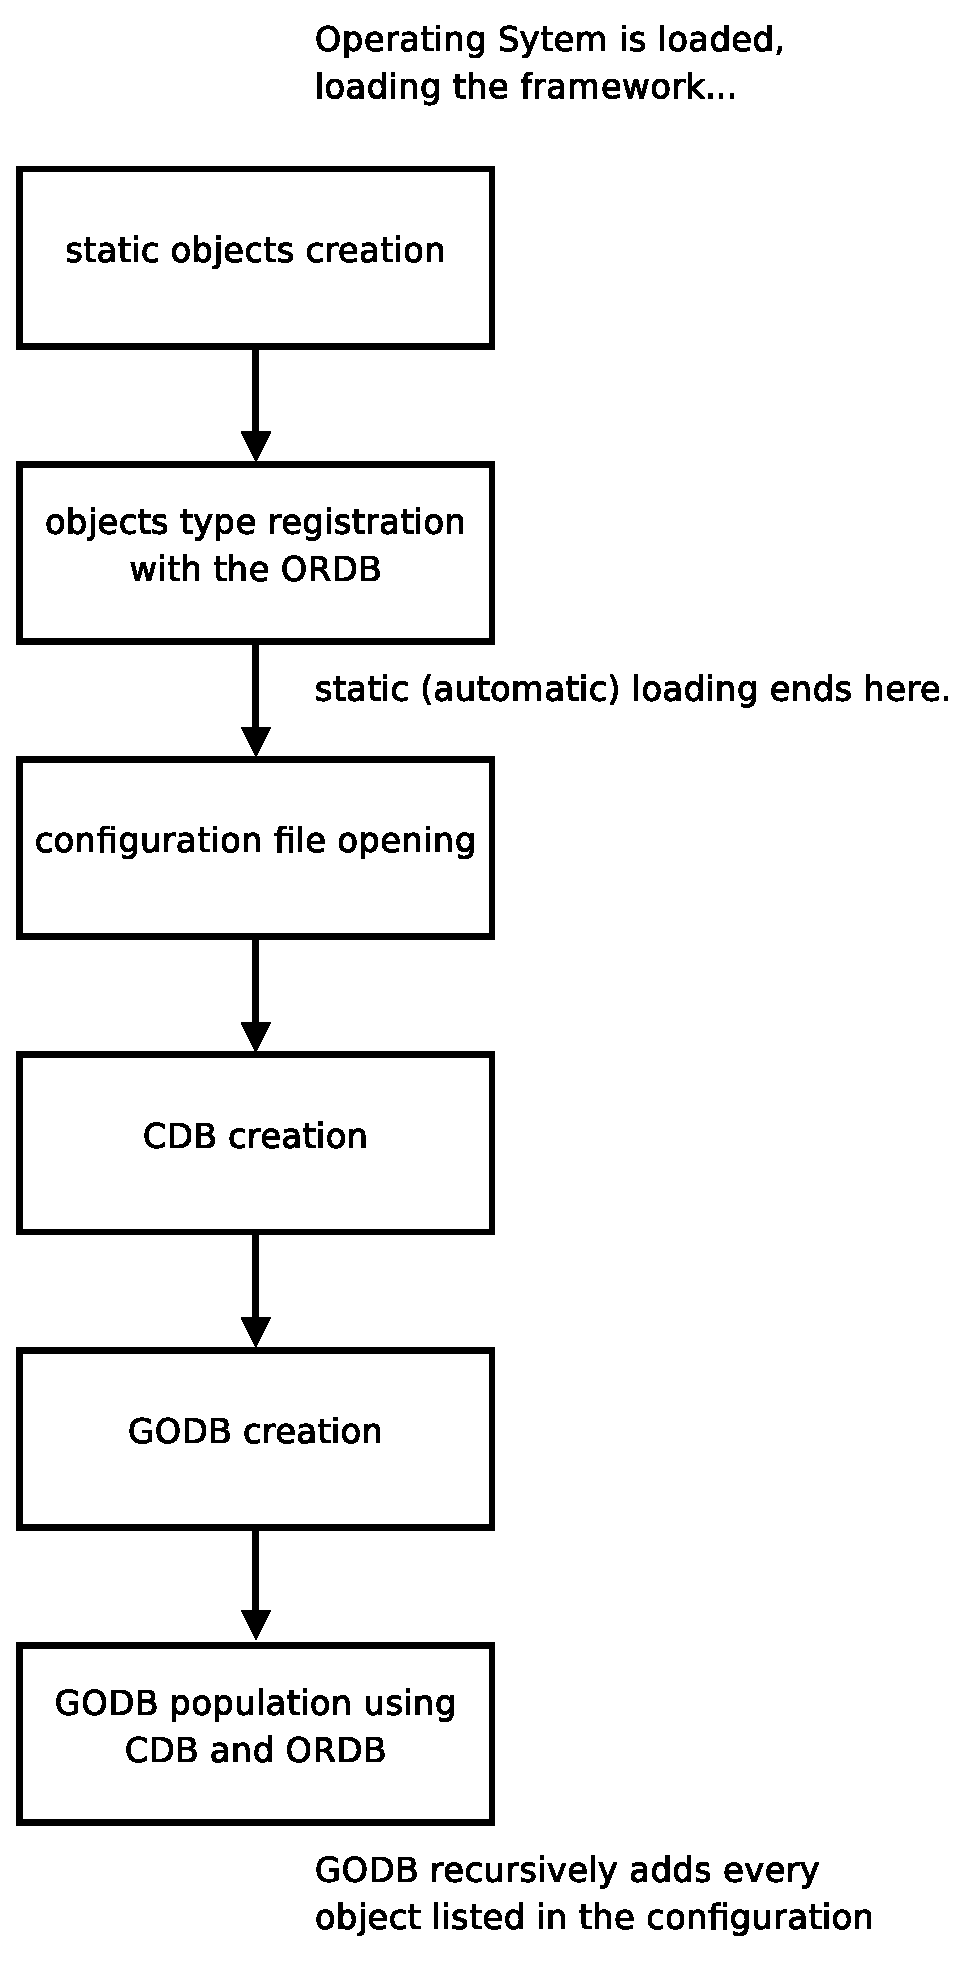
\includegraphics[width=0.33\textwidth]{level3/objects.eps}
  \caption{BaseLib objects loading and instantiation sequence}
  \label{f:level3:objects}
 \end{center}
\end{figure}



\paragraph{Example}
We now have a look to a simple example that make use of BaseLib and instantiate its objects via the CDB, the example is located in \textit{BaseLibTests/TestMessageBroker.cpp}. The first thing that follow is a snippets of a C++ source where there is the configuration data as a \texttt{char*} string. Don't try to understand what kind of objects are represented, they are no meaning in this place, have a look to the string format and try to understand the insights.

\begin{lstlisting}[
extendedchars=true,%
basicstyle=\fontfamily{pcr}\fontseries{m}\selectfont\footnotesize, %
stepnumber=1,%
numberstyle=\tiny,%
keywordstyle=\footnotesize\tt ,%
language=C++]
const char* testMessageBroker=
   "+TREES={"
   "    Class = GCReferenceContainer\n"
   "   +BRANCH1={\n"
   "        Class = GCReferenceContainer\n"
   "       +EP1={\n"
   "           Class = MessageEndPoint\n"
   "       }\n"
   "   }\n"
   "   +BRANCH2={\n"
   "        Class = GCReferenceContainer\n"
   "       +EP2={\n"
   "           Class = MessageEndPoint\n"
   "       }\n"
   "   }\n"
   "   +BRANCH3={\n"
   "        Class = MessageBroker\n"
   "        PeerIpAddress = localhost\n"
   "        PeerPort = 8882\n"
   "   }\n"
   "}\n"
   "+MC={\n"
   "    Class = MessageSenderTest\n"
   "}\n"
   "+MS={\n"
   "    Class = MessageServer\n"
   "    ServerPort = 8881\n"
   "}\n";
\end{lstlisting}

Now we follow the process of the objects creation starting from the previous string configuration. All the process, in the source behind is depicted, using a UML diagram, in Figure \ref{f:level3:TestMessageBroker}. The basic steps are: creating a stream of data, in this case an \texttt{SXMemory} object, create a \texttt{ConfigurationDataBase} object, that is a \texttt{GRTemplate} templatized on any \texttt{CDBVirtual}, in this case a \texttt{CDB} that we will analize in this chapter and then the \texttt{cdb} is passed to the GODB for class instantiation.

\begin{lstlisting}[
extendedchars=true,%
basicstyle=\fontfamily{pcr}\fontseries{m}\selectfont\footnotesize, %
stepnumber=1,%
numberstyle=\tiny,%
keywordstyle=\footnotesize\tt ,%
language=C++]
   SXMemory config((char*)testMessageBroker,strlen(testMessageBroker));
   ConfigurationDataBase cdb;
   if(!cdb->ReadFromStream(config,NULL)){
      CStaticAssertErrorCondition(ParametersError,"Init: cdb.ReadFromStream failed");
      return -1;
   }

   GCRTemplate<GCReferenceContainer> godb = GetGlobalObjectDataBase();
   godb->ObjectLoadSetup(cdb,NULL);
\end{lstlisting}

Creating a automatic class \texttt{ConfigurationDataBase} as we can see in Figure \ref{f:level3:TestMessageBroker}, let an automatic chain of constructor take place that construct defaulty a ConfigurationDataBase of type \texttt{CDB} that is the first issue addressed in this chapter.
\begin{figure}[h!]
 \begin{center}
  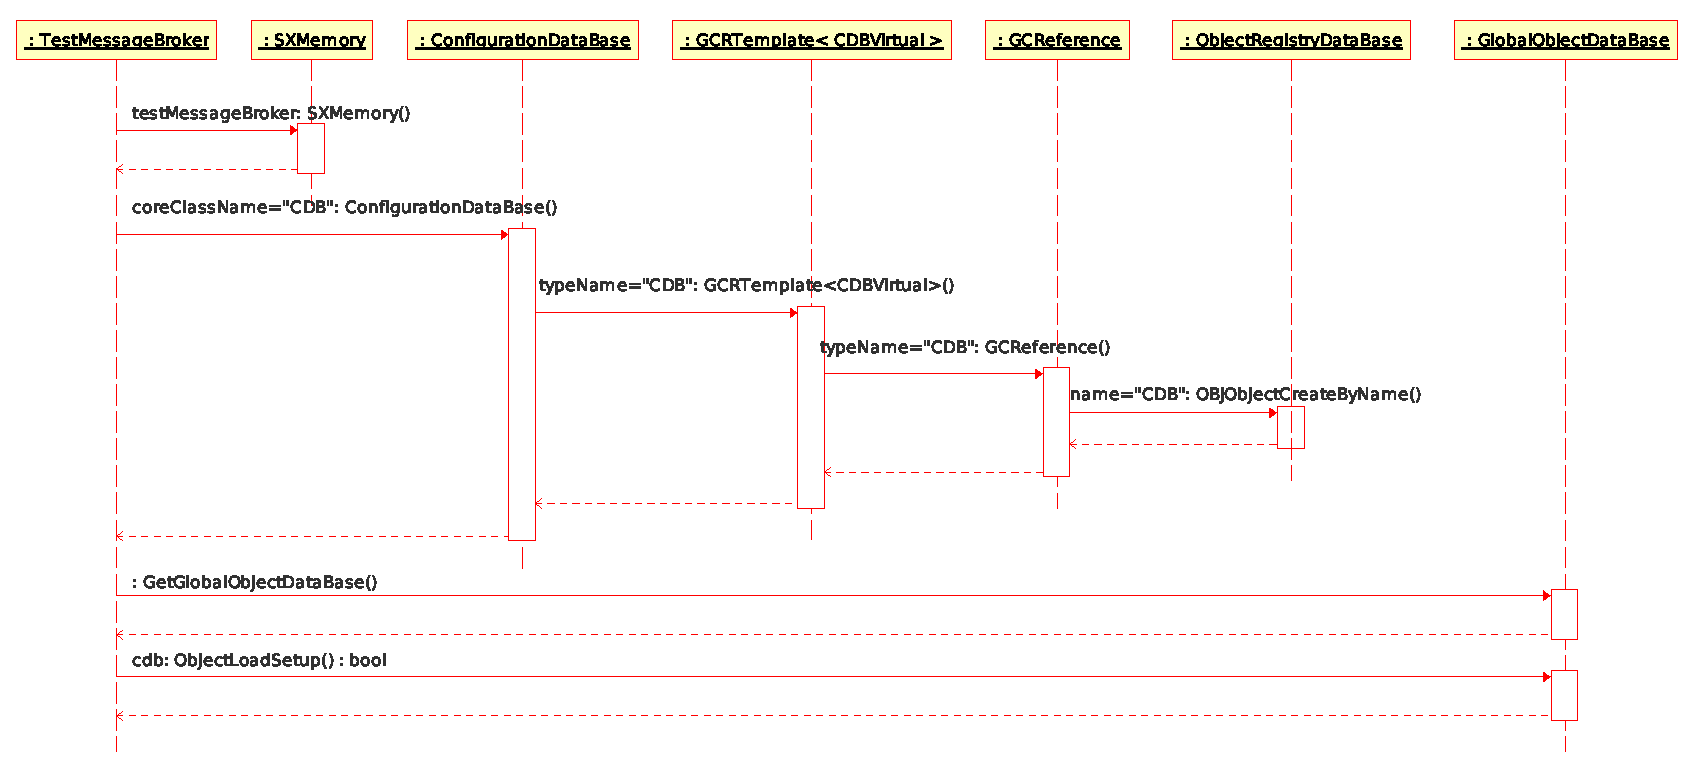
\includegraphics[width=\textwidth]{level3/TestMessageBroker.eps}
  \caption{BaseLib TestMessageBroker example}
  \label{f:level3:TestMessageBroker}
 \end{center}
\end{figure}

We end this introductory paragraph with another example of a configuration file. Those lines can be cut and pasted in a single file ending in \texttt{.cfg}.
\begin{lstlisting}[
extendedchars=true,%
basicstyle=\fontfamily{pcr}\fontseries{m}\selectfont\footnotesize, %
stepnumber=1,%
numberstyle=\tiny,%
keywordstyle=\footnotesize\tt ,%
language=bash]
+HttpServer = {
   Class = HttpService
   Port = 8084
}
+Control = {
   Class = ControlGAM
   Controller = {
      NoPlasmaVelocityGain = 0.0
      NoPlasmaCurrentGain = 40.0
         IPWaveform = {
            Times = {0 120}
            Amplitudes = {0.5 0.5}
            Rounding = 50
         }
   }
}
+DAM = {
   Class = DAMGAM
   // Projection matrix
   ProjectionMatrix = {
      0 = { 1.0 0.0 0.0 0.0 }
      1 = { 0.0 1.0 0.0 0.0 }
      2 = { 0.0 0.0 1.0 0.0 }
      3 = { 0.0 0.0 0.0 1.0 }
   }
}
\end{lstlisting}



\section{CDB}

We have just spend some words about the \texttt{Configuration Database} that will be presented in this section, this is the first real implementation of a CDB that inherits from the class \texttt{CDBVirtual}. Figure \ref{f:level3:CDB-exp} depict the UML diagram behind the classes in this section.

\begin{figure}[h!]
 \begin{center}
  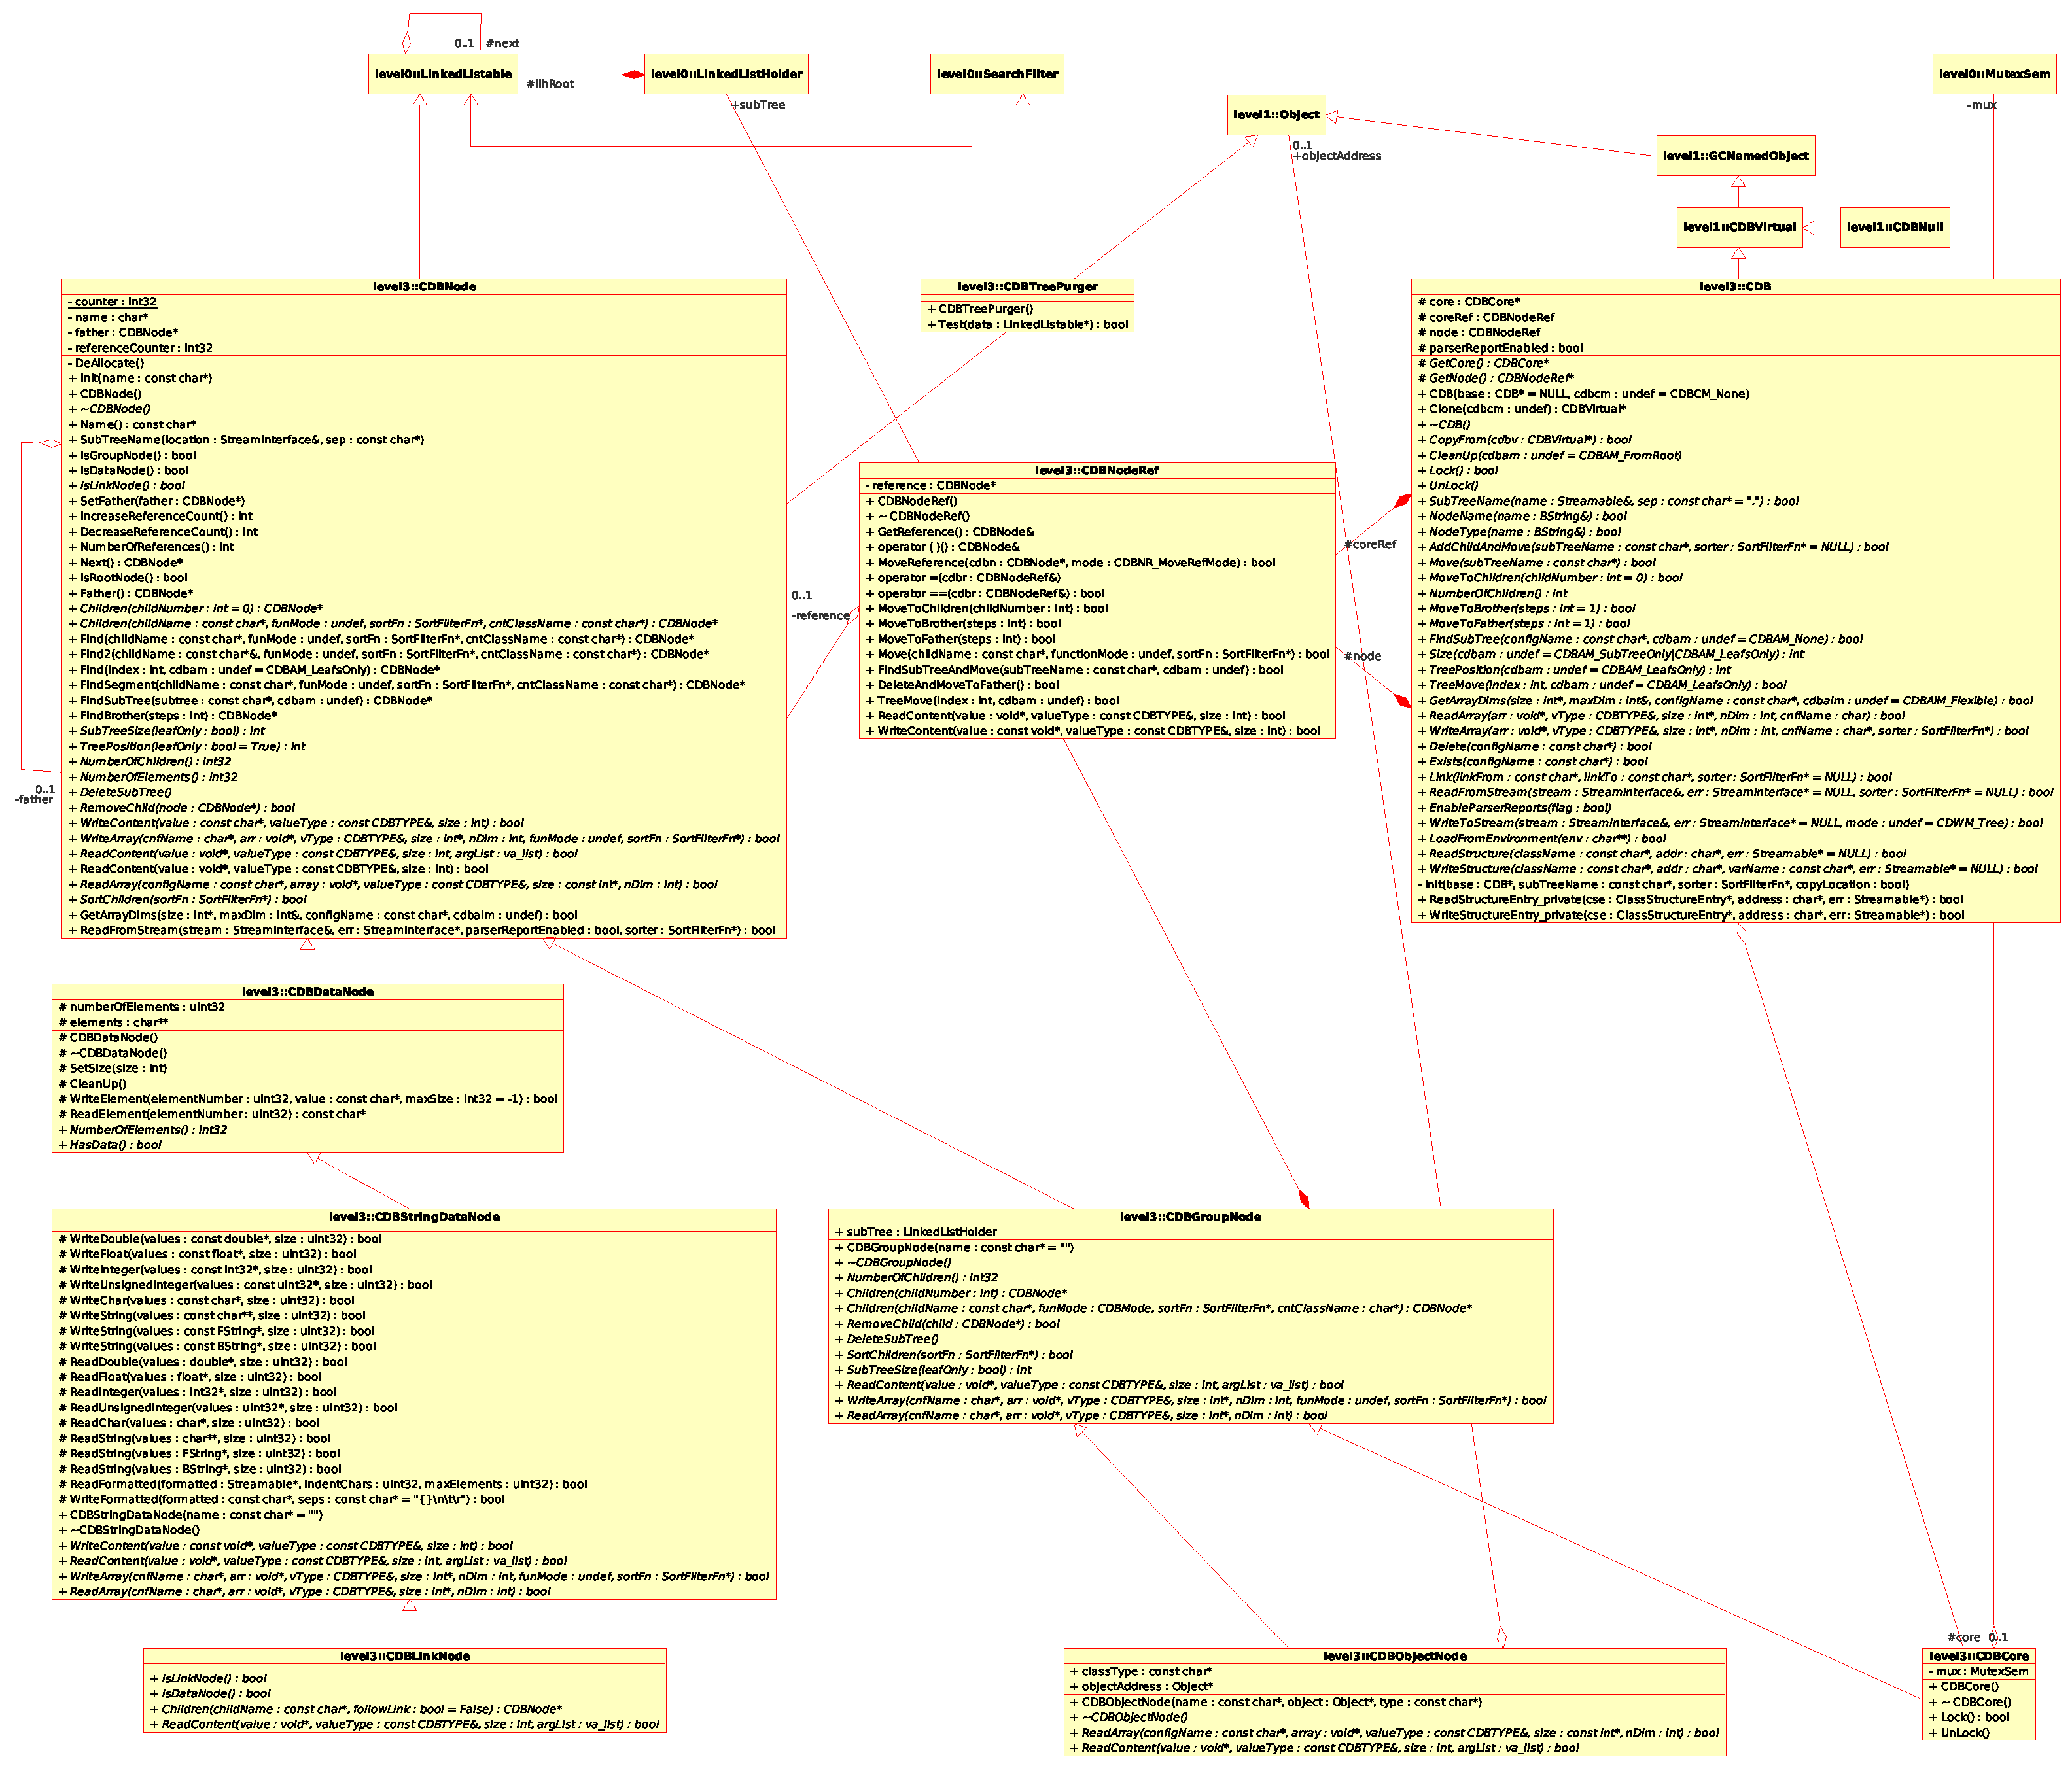
\includegraphics[width=1.1\textwidth]{level3/level3-CDB-exp.eps}
  \caption{BaseLib Level3 CDB (a Configuration Database implementation)}
  \label{f:level3:CDB-exp}
 \end{center}
\end{figure}

Class in this section are listed below.
\begin{itemize}
 \item CDBNode
 \item CDBDataNode
 \item CDBStringDataNode
 \item CDBLinkNode
 \item CDBGroupNode
 \item CDBObjectNode
 \item CDBCore
 \item CDBNodeRef
 \item CDB
 \item CDBCInterface
 \item CDBTreePurger
 \item CDBDataTypeInterface
\end{itemize}

The CDB tree data structure is designed with two basic data structures: leafs and internal nodes. Each internal node has at least a leaf (or another internal node). An internal node is a \texttt{CDBroupNode} and a leaf is a \texttt{CDBDataNode}. Figure \ref{f:level3:cdb-tree} depicts the structure described.

\begin{figure}[h!]
 \begin{center}
  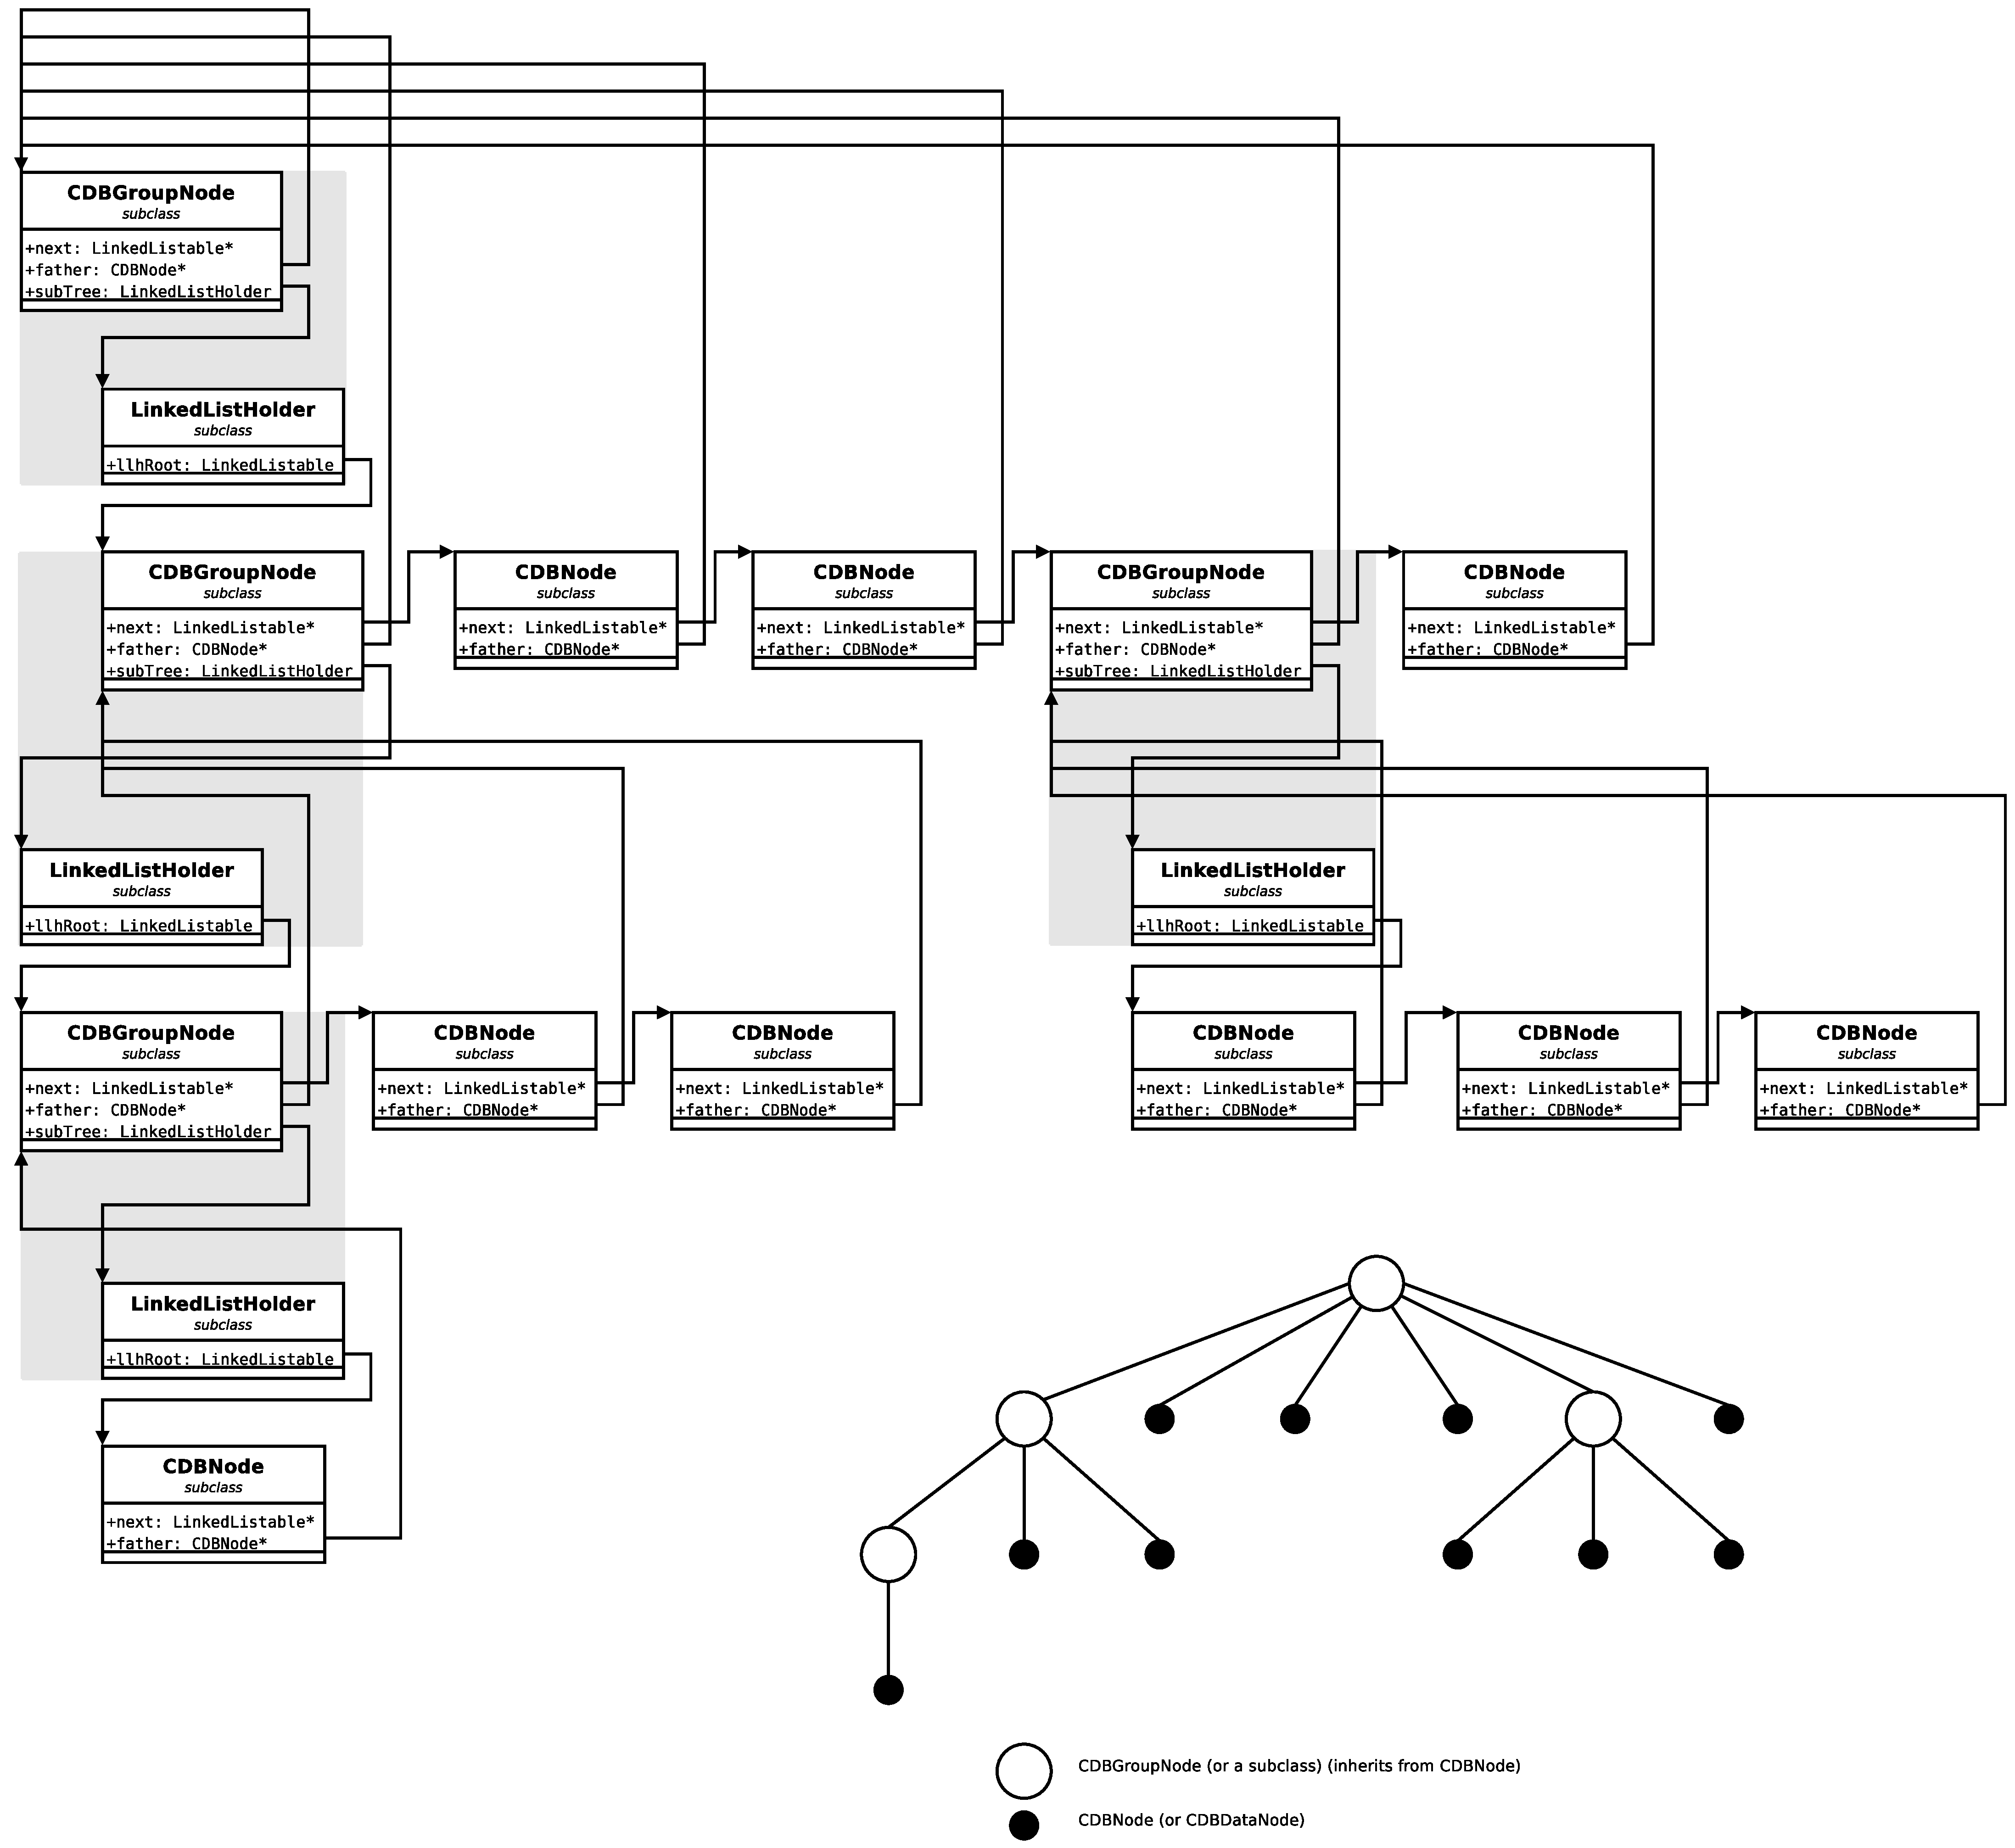
\includegraphics[width=\textwidth]{level3/CDB.eps}
  \caption{BaseLib Level3 CDB tree implementation}
  \label{f:level3:cdb-tree}
 \end{center}
\end{figure}



\subsubsection{CDBNode}
\texttt{[CDBNode.h, CDBNode.cpp]}\\
The class \texttt{CDBNode} is the basic node interface of the CDB tree data structure. Each type of node is build up the \texttt{CDBNode} class. In Figure \ref{f:level3:cdb-tree} the tree data structure of a CDB is depicted, each class is a \texttt{CDBNode} or a derived class of a \texttt{CDBNode}, class \texttt{level0::LinkedListHolder} is necessary to hold a linked list of \texttt{CDBNode} objects (of type \texttt{LinkedListable}).\\


We now switch to speak about attributes and methods of the \texttt{CDBNode} class. A \texttt{CDBNode} as the first attribute has a \texttt{static} \texttt{counter}, this variable lets hold the total number of nodes there are in the system, i.e. in the CDB, the constructor increment it and the deconstructor decrement it. Every node has a \texttt{name} that is really the name of the field, an object that it is its \texttt{father} in the tree and a \texttt{referenceCounter}, each node has its own \texttt{referenceCounter} for coherent destruction.
\begin{lstlisting}[
extendedchars=true,%
basicstyle=\fontfamily{pcr}\fontseries{m}\selectfont\footnotesize, %
stepnumber=1,%
numberstyle=\tiny,%
keywordstyle=\footnotesize\tt ,%
language=C++]
private:
   static int32 counter;

   char* name;
   CDBNode* father;
   int32 referenceCounter;
\end{lstlisting}

The first method we analysed is the private \texttt{DeAllocate} it deallocates memory used in a node (\texttt{name} allocated buffer); \texttt{Init} is public and inits the node and adds a name to it, then came the constructor and the destructor, that removes the node from its container also. \\


The method \texttt{Name} gets the \texttt{name} attribute of the class and \texttt{NumberOfElements} returns \texttt{-1} because such function must return how much data elements are contained by this node but a \texttt{CDBNode} is an abstraction of two node types so if is a leaf doesn't have elements but if it is an internal node it must have it. In this case it returns \texttt{-1} as an error, this function must be implemented at subclasses level. \\


The method \texttt{IsRootNode} check if the node is the root node of the tree, i.e. is a root node if the \texttt{father} attribute points to itself (is the same as the \texttt{this} pointer).
The method \texttt{IsGroupNode} in this case return \texttt{false} bacause only the subclass \texttt{CDBGroupNode} and derived return \texttt{true}; method \texttt{IsDataNode} returns \texttt{false} because \texttt{CDBNode} is not a \texttt{CDBDataNode} or a subclass of it. The methods \texttt{IsLinkNode()} return \texttt{true} whether it is a link to a different subtree, in the case of a \texttt{CDBNode} simply return \texttt{false}. \\


Methods \texttt{IncreaseReferenceCount}, \texttt{DecreaseReferenceCount} and \texttt{NumberOfReferences} increment, decrement and return atomically the attribute \texttt{referenceCounter}, such attribute show the number of users of this node. 
The method \texttt{Next} gets the next node, method \texttt{Father} gets the father of the node that you can sets via the method \texttt{SetFather}.
\begin{lstlisting}[
extendedchars=true,%
basicstyle=\fontfamily{pcr}\fontseries{m}\selectfont\footnotesize, %
stepnumber=1,%
numberstyle=\tiny,%
keywordstyle=\footnotesize\tt ,%
language=C++]
   void DeAllocate();
public:
   void Init(const char* name);

   CDBNode();
   virtual ~CDBNode();

   const char* Name() const;
   virtual int32 NumberOfElements() const;

   bool IsRootNode() const;
   inline bool IsGroupNode() const;
   inline bool IsDataNode() const;
   virtual bool IsLinkNode() const;

   int IncreaseReferenceCount();
   int DecreaseReferenceCount();
   int NumberOfReferences() const;

   CDBNode* Next() const;
   CDBNode* Father() const;
   void SetFather(CDBNode* father);
\end{lstlisting}

The first \texttt{Find} method finds a location within the whole (sub)tree as the object invoked on; remember that nodes are nombered from left to right and from subnode to supernode, if the node does not exist returns \texttt{false} and remains in the start position.

The second \texttt{Find} method simply call \texttt{Find2} method that has a sligtly different argument signature. \texttt{Find2} moves recursively in the tree from current position; \texttt{childName} can also be ``UpNode'' if you search is one level up, or ``RootNode'' if it is all the way up. Any movement onto unexisting subtree will fail; any movement out of unexisting subtree will erase temporary holders; movement is relative to current location. \texttt{childName} is returned modified to reflect the depth of matching.

The method \texttt{FindSegment} moves one level in the tree, we must remember that the CDB is a configuration tree that holds configuration data, as \texttt{Find2} \texttt{childName} argument if ``UpNode'' means one level up and if means ``RootNode'' is all the way up; as before any movement onto unexisting subtree will fail,any movement out of unexisting subtree will erase temporary holders; movement is relative to current location.
The method \texttt{FindSubTree}  moves to a node pointing to the specified subtree. \texttt{FindBrother} allows accessing brothers; negative and positive numbers allow to move relative to start position. \\


The method \texttt{SubTreeName} returns the name of the subtree starting from this node, this call is safe, does not require locking of tree. \texttt{SubTreeSize} returns \texttt{1} for a \texttt{CDBNode}, subclass of such class returns different values. \texttt{DeleteSubTree} will remove all unreferenced subtrees, in \texttt{CDBNode} doesn't take any action. \texttt{TreePosition} returns the position of the node within the tree. \\


The method \texttt{NumberOfChildren} returns how many childrens of this node, \texttt{-1} means it is not a node that has children, in this implementation \texttt{CDBNode} returns \texttt{-1}. The first \texttt{Children} allows accessing the subtrees and uptrees (using negative indexes -1 -2), \texttt{CDBNode} implements only access to uptrees. Second \texttt{Children} method allows accessing the subtrees by name, \texttt{childName} is the name of the node, it cannot be a full subtree; \texttt{functionMode} is of type \texttt{CDBNMode}, argument \texttt{sortFn} is used only if adding a node; this method is not implemented in \texttt{CDBNode} and simply return \texttt{NULL}. \texttt{SortChildren} apply sorting to the subtree; \texttt{RemoveChild} removes the specified child if exists.
\begin{lstlisting}[
extendedchars=true,%
basicstyle=\fontfamily{pcr}\fontseries{m}\selectfont\footnotesize, %
stepnumber=1,%
numberstyle=\tiny,%
keywordstyle=\footnotesize\tt ,%
language=C++]
   CDBNode* Find(int index,CDBAddressMode cdbam=CDBAM_LeafsOnly);
   inline CDBNode* Find(const char* childName,CDBNMode functionMode=CDBN_None,
      SortFilterFn* sortFn=NULL,const char* containerClassName=NULL);
   CDBNode* Find2(const char*& childName,CDBNMode functionMode=CDBN_None,
      SortFilterFn* sortFn=NULL,const char* containerClassName=NULL);
   CDBNode* FindSegment(const char* childName,CDBNMode functionMode=CDBN_None,
      SortFilterFn* sortFn=NULL,const char* containerClassName=NULL);
   CDBNode* FindSubTree(const char* subtree,CDBAddressMode cdbam);
   CDBNode* FindBrother(int steps);

   void SubTreeName(Streamable& location, const char* sep);
   virtual int SubTreeSize(bool leafOnly);
   virtual void DeleteSubTree();
   virtual int TreePosition(bool leafOnly = True);

   virtual int32 NumberOfChildren() const;
   virtual CDBNode* Children(int childNumber=0);
   virtual CDBNode* Children(const char* childName,CDBNMode functionMode=CDBN_SearchOnly,
      SortFilterFn* sortFn=NULL,const char* containerClassName=NULL);
   virtual bool SortChildren(SortFilterFn* sortFn);
   virtual bool RemoveChild(CDBNode* node);
\end{lstlisting}

Methods \texttt{WriteContent}, \texttt{WriteArray}, \texttt{ReadContent} and \texttt{ReadArray} are all implemented in subclasses and in the class \texttt{CDBNode} simply return \texttt{false}. Read and write methods are implemented in \texttt{CDBDataNode} and subclasses.\\


The method \texttt{GetArrayDim} reads the dimensions of a matrix, it expects all the indexes to be found form $0$ to $N$. \texttt{ReadFromStream} parses the stream and build a configuration database according to the simple CDB syntax. Those methods are implemented in \texttt{CDBNode}.
\begin{lstlisting}[
extendedchars=true,%
basicstyle=\fontfamily{pcr}\fontseries{m}\selectfont\footnotesize, %
stepnumber=1,%
numberstyle=\tiny,%
keywordstyle=\footnotesize\tt ,%
language=C++]
   virtual bool WriteContent(const void* value,const CDBTYPE& valueType,int size);
   virtual bool WriteArray(const char* configName,const void* array,
      const CDBTYPE& valueType,const int* size,int nDim,
      CDBNMode functionMode=CDBN_CreateStringNode,SortFilterFn* sortFn=NULL);

   virtual bool ReadContent(void* value,const CDBTYPE& valueType,
      int size,va_list argList);
   bool ReadContent(void* value,const CDBTYPE& valueType,int size,...);
   virtual bool ReadArray(const char* configName,void* array,
      const CDBTYPE& valueType,const int* size,int nDim);

   bool GetArrayDims(int* size,int& maxDim,const char* configName,
      CDBArrayIndexingMode cdbaim);
   bool ReadFromStream(StreamInterface& stream,StreamInterface* err,
      bool parserReportEnabled,SortFilterFn* sorter);
\end{lstlisting}



\subsubsection{CDBDataNode}
\texttt{[CDBStringDataNode.h, CDBStringDataNode.cpp]}\\
The class \texttt{CDBDataNode} is the low level abstraction of all nodes containing data. It basically adds few methods and ttributes to the \texttt{CDBNode} class. \\


The first attribute \texttt{numberOfElements} can be $1$ if the other attribute, \texttt{elements}, points to a string directly; greater then $1$ if \texttt{elements} is a pointer to an array of pointers.
As we said \texttt{elements} is a vector of pointers or a direct pointer to data if \texttt{numberOfElements} is $1$, if \texttt{numberOfElements} is $0$ \texttt{elements} should be \texttt{NULL}. \\


Constructor set \texttt{elements} to \texttt{NULL} and \texttt{numberOfElements} to $0$; deconstructor call the method \texttt{CleanUp}.

The method \texttt{SetSize} resize data structure, i.e. it will call malloc on the attribute \texttt{elements} and copies the old data. \texttt{CleanUp} frees each elements and turn the data structure to $0$ elemnts like the constructor.

The method \texttt{WriteElement} adds a new element in the \texttt{elements} array, such function handle also allocation of the memory, with the \texttt{ReadElement} method is also possible to read the entry just written.

The method \texttt{NumberOfElements} simply return the attribute \texttt{NumberOfElements}, i.e. how much data elements are contained by this node, $-1$ means it is not a node that has data. \texttt{HasData} return \texttt{true} whether it is to be considered a leaf node.
\begin{lstlisting}[
extendedchars=true,%
basicstyle=\fontfamily{pcr}\fontseries{m}\selectfont\footnotesize, %
stepnumber=1,%
numberstyle=\tiny,%
keywordstyle=\footnotesize\tt ,%
language=C++]
protected:
   uint32 numberOfElements;
   char** elements;

   CDBDataNode();
   ~CDBDataNode();

   void SetSize(int size);
   void CleanUp();
   bool WriteElement(uint32 elementNumber,const char* value,int32 maxSize=-1);
   const char* ReadElement(uint32 elementNumber) const;

   virtual int32 NumberOfElements() const;
   virtual bool HasData() const;
\end{lstlisting}



\subsubsection{CDBStringDataNode}
\texttt{[CDBStringDataNode.h, CDBStringDataNode.cpp]}\\
The class \texttt{CDBStringDataNode} is a csubclass of a \texttt{CDBDataNode} that holds data in string format, it is possible to convert from a string to each other type. Obviously if a string is a character array of letters can't be converted in a double. The class provides no attributes. \\


Following methods write (it makes a copy) of respectively double, float, integer, unsigned integer, char and strings from the first argument to the \texttt{CDBDataNode::elements} pointer. Each method accept in input not only one value but an array of data with the same format. Read methods have the same behaviour but copy the \texttt{elements} pointer to the \texttt{values} argument.
All the write methods make use of the superclass method's \texttt{CDBDataNode::WriteElement} and write methods of \texttt{CDBDataNode::ReadElement}.
\begin{lstlisting}[
extendedchars=true,%
basicstyle=\fontfamily{pcr}\fontseries{m}\selectfont\footnotesize, %
stepnumber=1,%
numberstyle=\tiny,%
keywordstyle=\footnotesize\tt ,%
language=C++]
protected:
   bool WriteDouble(const double* values,uint32 size);
   bool WriteFloat(const float* values,uint32 size);
   bool WriteInteger(Const int32* values,uint32 size);
   bool WriteUnsignedInteger(const uint32* values,uint32 size);
   bool WriteChar(const char* values,uint32 size);
   bool WriteString(const char** values,uint32 size);
   bool WriteString(const FString* values,uint32 size);
   bool WriteString(const BString* values,uint32 size);

   bool ReadDouble(double* values,uint32 size);
   bool ReadFloat(float* values,uint32 size);
   bool ReadInteger(int32* values,uint32 size);
   bool ReadUnsignedInteger(uint32* values,uint32 size);
   bool ReadChar(char* values,uint32 size);
   bool ReadString(char** values,uint32 size);
   bool ReadString(FString* values,uint32 size);
   bool ReadString(BString* values,uint32 size);
\end{lstlisting}

The method \texttt{WriteFormatted} takes a formatted string as an input and write it in the texttt{CDBDataNode::elements} attribute; probably the formatted input can contain data of different type. The method \texttt{ReadFormatted} read outputting on the \texttt{Streamable} argument all the elements in the \texttt{CDBDataNode} array, inserting ${}$ around the formatted stream.
\begin{lstlisting}[
extendedchars=true,%
basicstyle=\fontfamily{pcr}\fontseries{m}\selectfont\footnotesize, %
stepnumber=1,%
numberstyle=\tiny,%
keywordstyle=\footnotesize\tt ,%
language=C++]
   bool WriteFormatted(const char* formatted,const char* seps=" {}\n\t\r");
   bool ReadFormatted(Streamable* formatted,uint32 indentChars,uint32 maxElements);
\end{lstlisting}

Now comes public methods. The method \texttt{WriteContent} writes data on a node the value can be of any \texttt{CDBTYPE} the \texttt{size} argument specifies how many elements. The class \texttt{CDBTYPE} is declared in \textit{level1}. Table shows registered \texttt{CDBTYPE}s, from \textit{level1/CDBTypes.h}.

\begin{table}[!h]
 \begin{center}
  \begin{tabular}{|l|l|l|}
   \hline
name & CDBDataType & sizeof() \\
    \hline
\texttt{CDBTYPE\_float} & \texttt{CDB\_float} & \texttt{float} \\
\texttt{CDBTYPE\_double} & \texttt{CDB\_double} & \texttt{double} \\
\texttt{CDBTYPE\_int32} & \texttt{CDB\_int32} & \texttt{int32} \\
\texttt{CDBTYPE\_uint32} & \texttt{CDB\_uint32} & uint32 \\
\texttt{CDBTYPE\_char} & \texttt{CDB\_char} & \texttt{char} \\
\texttt{CDBTYPE\_hex} & \texttt{CDB\_hex} & \texttt{uint32} \\
\texttt{CDBTYPE\_octal} & \texttt{CDB\_octal} & \texttt{uint32} \\
\texttt{CDBTYPE\_String} & \texttt{CDB\_String} & \texttt{char*} \\
\texttt{CDBTYPE\_BString} & \texttt{CDB\_BString} & \texttt{BString} \\
\texttt{CDBTYPE\_NULL} & \texttt{CDB\_None} & \texttt{NULL} \\
    \hline
    \end{tabular}
   \end{center}
  \caption{Level1 declared \texttt{CDBTYPE}s in \textit{level1/CDBTypes.h} }
 \label{t:level1:CDBTYPE}
\end{table}

\texttt{ReadContent} reads data from a node, \texttt{valueType} specifies data type, \texttt{size} specifies how many elements and \texttt{value} contains a pointer to memory where to write the data.

The method \texttt{WriteArray} writes content (one to many elements) into a data node, creates a data node or modifies an existing, \texttt{configName} is the address of the parameter relative to the current node, \texttt{array} is the data in whatever form specified by \texttt{valueType} and \texttt{size} is a vector of matrix dimensions; if \texttt{size} is \texttt{NULL} it treats the input as a monodimensional array of size \texttt{nDim}; \texttt{sortFn} allows inserting newly created nodes in a specific order.
The method \texttt{ReadArray} reads content from a data node to the \texttt{configName} pointer argument.
\begin{lstlisting}[
extendedchars=true,%
basicstyle=\fontfamily{pcr}\fontseries{m}\selectfont\footnotesize, %
stepnumber=1,%
numberstyle=\tiny,%
keywordstyle=\footnotesize\tt ,%
language=C++]
public:
   CDBStringDataNode(const char* name="");
   ~CDBStringDataNode();

   virtual bool WriteContent(const void* value,const CDBTYPE& valueType,int size);
   virtual bool ReadContent(void* value,const CDBTYPE& valueType,int size,va_list argList);

   virtual bool WriteArray(const char* configName,const void* array,
      const CDBTYPE& valueType,const int* size,int nDim,
      CDBNMode functionMode=CDBN_CreateStringNode,SortFilterFn* sortFn=NULL);
   virtual bool ReadArray(const char* configName,void* array,
      const CDBTYPE& valueType,const int* size,int nDim);
\end{lstlisting}



\subsubsection{CDBLinkNode}
\texttt{[CDBLinkNode.h, CDBLinkNode.cpp]}\\
Such \texttt{CDBLinkNode} should implements hard link between nodes. The constructor calls the superclass constructor, this class is a subclass of a \texttt{CDBStringDataNode}. \\


Methods \texttt{IsLinkNode} and \texttt{IsDataNode} return \texttt{true} each.
\texttt{Children} allows accessing the subtrees by name but in this case simply return \texttt{NULL}; if argument \texttt{followLink} is \texttt{true} links are followed.
\texttt{ReadContent} reads data from a node, this is the only real method implemented, it should find what to read in the \texttt{value} argument and then treat the same argument as an output stream. Not really well implemented.
\begin{lstlisting}[
extendedchars=true,%
basicstyle=\fontfamily{pcr}\fontseries{m}\selectfont\footnotesize, %
stepnumber=1,%
numberstyle=\tiny,%
keywordstyle=\footnotesize\tt ,%
language=C++]
public:
   CDBLinkNode(const char *name);
   virtual bool IsLinkNode() const;
   virtual bool IsDataNode() const;
   virtual CDBNode* Children(const char* childName,bool followLink=False);
   virtual bool ReadContent(void* value,const CDBTYPE& valueType,int size,va_list argList);
\end{lstlisting}



\subsubsection{CDBGroupNode}
\texttt{[CDBGroupNode.h, CDBGroupNode.cpp]}\\
A CDB tree is constituited of two basic types of nodes: \texttt{CDBDataNode} and \texttt{CDBGroupNode} respectively leafs and internal nodes. Internal nodes are \texttt{CDBGroupNode} and basically are containers of \texttt{CDBNode}s, i.e. the branches of the tree. So the only, but the most important, attribute of this class is \texttt{subTree} a \texttt{LinkedListHolder} that holds all the nodes underneath in the tree.
\begin{lstlisting}[
extendedchars=true,%
basicstyle=\fontfamily{pcr}\fontseries{m}\selectfont\footnotesize, %
stepnumber=1,%
numberstyle=\tiny,%
keywordstyle=\footnotesize\tt ,%
language=C++]
public:
   LinkedListHolder subTree;
\end{lstlisting}

The constructor invokes the superclass's constructor with the passed by name; destructor call \texttt{LinkedListHolder::Reset} method. \texttt{NumberOfChildren} returns the number of elements contained in the linked list of the attribute, i.e. the number of children of this node.
The first \texttt{Children} method allows accessing the subtrees and uptrees (with negative values, -1 -2...),the links are not expanded by this function; second \texttt{Children} method allows accessing the subtrees by name, \texttt{childName} is the name of the node, it cannot be a full subtree; \texttt{followLink} if \texttt{true} links are followed, \texttt{sortFn} used only if adding a node.
The method \texttt{RemoveChild} removes a child by name; \texttt{DeleteSubTree} removes all unreferenced subtrees; \texttt{SortChildren} apply sorting. \texttt{SubTreeSize} returns how many elements in the sub tree, note that is far different from \texttt{NumberOfChildren} because counts elements in all the sub tree from the node.
\begin{lstlisting}[
extendedchars=true,%
basicstyle=\fontfamily{pcr}\fontseries{m}\selectfont\footnotesize, %
stepnumber=1,%
numberstyle=\tiny,%
keywordstyle=\footnotesize\tt ,%
language=C++]
public:
   CDBGroupNode(const char* name="");
   virtual ~CDBGroupNode();

   virtual int32 NumberOfChildren() const;
   virtual CDBNode* Children(int childNumber);
   virtual CDBNode* Children(const char* childName,
      CDBNMode functionMode=CDBN_SearchOnly,SortFilterFn* sortFn=NULL,
      const char* containerClassName=NULL);
   virtual bool RemoveChild(CDBNode* child);
   virtual void DeleteSubTree();
   virtual bool SortChildren(SortFilterFn* sortFn);
   virtual int SubTreeSize(bool leafOnly);
\end{lstlisting}

Methods that follow are just be analysed before and are not treated here. All those three methods, \texttt{ReadContent}, \texttt{WriteArray} and \texttt{ReadArray} are implemented here.
\begin{lstlisting}[
extendedchars=true,%
basicstyle=\fontfamily{pcr}\fontseries{m}\selectfont\footnotesize, %
stepnumber=1,%
numberstyle=\tiny,%
keywordstyle=\footnotesize\tt ,%
language=C++]
   virtual bool ReadContent(void* value,const CDBTYPE& valueType,
      int size,va_list argList);

   virtual bool WriteArray(const char* configName,const void* array,
      const CDBTYPE& valueType,const int* size,int nDim,�
      CDBNMode functionMode=CDBN_CreateStringNode,SortFilterFn* sortFn=NULL);
   virtual bool ReadArray(const char* configName,void* array,
      const CDBTYPE& valueType,const int* size,int nDim);
\end{lstlisting}



\subsubsection{CDBObjectNode}
\texttt{[CDBObjectNode.h, CDBObjectNode.cpp]}\\
From the sources it is possible to read that a \texttt{CDBObjectNode} is ``a container of CDBNodes and of an Object''; most important is that the \texttt{CDBObjectNode} class inherits from \texttt{CDBGroupNode} and has as attributes a \texttt{const char*} and a \texttt{Object*} so it has an \texttt{Object} associated with it. The constructor register the name of the node, the pointer to the object and also the class type as a string.\\


The method \texttt{ReadArray} reads content from a data node, \texttt{configName} is the address of the parameter relative to the current node, \texttt{array} is the data in wahtever form specified by \texttt{valueType}, \texttt{size} is a vector of matrix dimensions, if \texttt{size} is \texttt{NULL} it treats the input as a monodimensional array of size \texttt{nDim}; \texttt{nDim} specifies how many dimensions the array possesses or the vector size if \texttt{size} is \texttt{NULL}. \texttt{ReadContent} reads also data from a node argument \texttt{value} contains a pointer to memory where to write the data.
\begin{lstlisting}[
extendedchars=true,%
basicstyle=\fontfamily{pcr}\fontseries{m}\selectfont\footnotesize, %
stepnumber=1,%
numberstyle=\tiny,%
keywordstyle=\footnotesize\tt ,%
language=C++]
public:
   const char* classType;
   Object* objectAddress;

   CDBObjectNode(const char* name,Object* object,const char* type);
   virtual ~CDBObjectNode();

   virtual bool ReadArray(const char* configName,void* array,
      const CDBTYPE& valueType,const int* size,int nDim);
   virtual bool ReadContent(void* value,const CDBTYPE& valueType,
      int size,va_list argList);
\end{lstlisting}



\subsubsection{CDBCore}
\texttt{[CDBCore.h]}\\
Probably the class \texttt{CDBCore} is the most simplest class of \textit{level3}, it only use a \texttt{level0:MutexSem} guaranteeing shared access to a CDB context safe. The class code follow.
\begin{lstlisting}[
extendedchars=true,%
basicstyle=\fontfamily{pcr}\fontseries{m}\selectfont\footnotesize, %
stepnumber=1,%
numberstyle=\tiny,%
keywordstyle=\footnotesize\tt ,%
language=C++]
class CDBCore: public CDBGroupNode{
private:
   MutexSem mux;
public:
   CDBCore(){ mux.Create();}
   virtual ~CDBCore(){ }
   virtual bool Lock(){
      if (!mux.Lock()){
         CStaticAssertErrorCondition(FatalError,"CDBCore Lock failed!");
         return False;
      }
      return True;
   }
   virtual void UnLock(){
      mux.UnLock();
   }
};
\end{lstlisting}



\subsubsection{CDBNodeRef}
\texttt{[CDBNodeRef.h, CDBNodeRef.cpp]}\\
The class \texttt{CDBNodeRef} is a reference to a \texttt{CDBNode} that remaps some methods. The only attribute is infact a \texttt{CDBNode*}. The class is a kind of iterator to move between nodes.

The constructor takes no arguments and initialize the object to a dummy \texttt{CDBNode} reference. The distructor move the reference away. There is also a copy operator overridden and a compare operator redefinition.
\begin{lstlisting}[
extendedchars=true,%
basicstyle=\fontfamily{pcr}\fontseries{m}\selectfont\footnotesize, %
stepnumber=1,%
numberstyle=\tiny,%
keywordstyle=\footnotesize\tt ,%
language=C++]
   CDBNode* reference;
public:
   CDBNodeRef();
   ~CDBNodeRef();

   inline CDBNode &GetReference();
   inline CDBNode &operator();
   inline void operator=(CDBNodeRef &cdbr);
   inline bool operator==(CDBNodeRef &cdbr);
\end{lstlisting}

The method \texttt{MoveReference} changes the reference to the node, if argument \texttt{cdbn} is \texttt{NULL} than it will refer to the globally allocated \texttt{nullCDBNode}.

The method \texttt{MoveToChildren} allows accessing the subtrees (argument \texttt{childNumber>=0}) and uptree (-1, -2, -3, ...); \texttt{MoveToBrother} allows accessing the brothers and \texttt{MoveToFather} allows acceesing brothers.

The method \texttt{Move} is the general method that allows accessing the subtrees and uptrees, like in \texttt{CDBNode} ``UpNode'' is one level up and ``RootNode'' is all the way up, any movement onto unexisting subtree will fail; any movement out of unexisting subtree will erase temporary holders; finally movements are relative to current location. \\


The method \texttt{FindSubTreeAndMove} moves to a node pointing to the specified subtree; \texttt{DeleteAndMoveToFather} remove current node and move up, the operation will complete only if the number of users is 0, the up movement will happen anyway. \texttt{TreeMove} moves to a location within the whole (sub)tree. \\


The method \texttt{ReadContent} reads data on a node, \texttt{valueType} specifies data type and \texttt{size} specifies how many elements; \texttt{WriteContent} writes data on a node argument \texttt{valueType} specifies data type and \texttt{size} specifies how many elements.

\begin{lstlisting}[
extendedchars=true,%
basicstyle=\fontfamily{pcr}\fontseries{m}\selectfont\footnotesize, %
stepnumber=1,%
numberstyle=\tiny,%
keywordstyle=\footnotesize\tt ,%
language=C++]
   bool MoveReference( CDBNode *cdbn, CDBNR_MoveRefMode mode);
   inline bool MoveToChildren(int childNumber=0);
   inline bool MoveToBrother(int steps = 1);
   inline bool MoveToFather(int steps = 1);
   inline bool Move(const char* childName,CDBNMode functionMode=CDBN_None,
      SortFilterFn* sortFn=NULL);

   inline bool FindSubTreeAndMove(const char* subTreeName,
      CDBAddressMode cdbam=CDBAM_None);
   inline bool DeleteAndMoveToFather();
   inline bool TreeMove(int index,CDBAddressMode cdbam=CDBAM_LeafsOnly);

   bool ReadContent(void* value,const CDBTYPE& valueType,int size,...);
   inline bool WriteContent(const void* value,const CDBTYPE& valueType,int size);
\end{lstlisting}



\subsubsection{CDB}
\texttt{[CDB.h, CDB.cpp]}\\
Like a \texttt{CDBNull} a \texttt{CDB} class extends a \texttt{CDBVirtual}. A \texttt{CDB} is an implementation of a hierarchical database. It works similarly to a filesystem having directory nodes (internal nodes or branches) and file nodes (leaves).

Each leaf node (\texttt{CDBDataNode}) is a container of a sequence of characters, both ASCII and not ASCII. \texttt{CDB} is infact a reference to an instance of the database. Copying \texttt{CDB}s does not duplicate the database but increases a reference counter. Operation to the same database by different
threads is safe. \\


We start with the attributes as usual. The first attribute is a \texttt{CDBCore*} that is used to acquire concurrent access to a \texttt{CDB}, the first \texttt{CDBNodeRef} is a pointer to the root node of the \textit{Configuration DataBase}, second \texttt{CDBNodeRef} is a pointer to the current node, obviously it can point to branches or leaves. Last argument \texttt{parserReportEnabled} said whether parsing reports faults.

The method \texttt{GetCore} basically return the \texttt{core} attribute and \texttt{GetNode} return a reference to the \texttt{node} attribute.
\begin{lstlisting}[
extendedchars=true,%
basicstyle=\fontfamily{pcr}\fontseries{m}\selectfont\footnotesize, %
stepnumber=1,%
numberstyle=\tiny,%
keywordstyle=\footnotesize\tt ,%
language=C++]
protected:
   CDBCore* core;
   CDBNodeRef coreRef;
   CDBNodeRef node;
   bool parserReportEnabled;

   virtual CDBCore* GetCore();
   virtual CDBNodeRef* GetNode();
\end{lstlisting}

The first method is the constructor of a CDB, if \texttt{base} is specified it creates a new reference to an existing database; if \texttt{NULL} creates a new database; argument \texttt{cdbcm} must be \texttt{CDBCM\_CopyAddress} to copy the address from the reference; in case of two or more flags, after oring one must cast back to the enum type. \texttt{Clone} simply call the constructor with \texttt{this } as \texttt{base} argument creating a new reference to a database, or if that is not possible it creates a copy. Then comes the destructor that does nothing, but will destroy database if instance count goes to zero. The method \texttt{CopyFrom} copy all the \texttt{CDB} passed by to the current \texttt{CDB}. \texttt{CleanUp} removes all the content from the database unless some other database instance exists and points to a subtree one can request to delete only the current subtree. \\


The method \texttt{Lock} locks the main database for exclusive access: use if a group of transactions should be atomic, \texttt{UnLock} unlocks the main database: remember unlocking a locked database after use. \\


The method \texttt{SubTreeName} finds the overall path leading to the current node, \texttt{NodeName} returns the name of the current node and \texttt{NodeType} gets the type of the current node. \\


The method \texttt{AddChildAndMove} can be used to create a new subtree, \texttt{Move} moves the \texttt{node} attribute to the specified location, the movement is relative to the current location. \texttt{MoveToChildren} moves the \texttt{node} attribute, negative number move up, zero is the first of the children; \texttt{NumberOfChildren} returns how many branches there are from this node; negative number implies that the location is a leaf. The method \texttt{MoveToBrother} moves to a brother's node, with $0$ means remain where you are, greater then $0$ brothers on the right below $0$ on the left.
\texttt{MoveToFather} moves up, \texttt{-1} means \texttt{Root}, one level up for each positive. \\


The method \texttt{FindSubTree} search a node identified by \texttt{configName} attribtue from node search on the right of the tree for the subtree identified by the string name, on success \texttt{node} attribute points to the node containing the subtree or leaf, such method will not follow links.
\texttt{Size} return the total number of nodes, param \texttt{cdbam} if \texttt{CDBAM\_SubTreeOnly} allows to measure the current subtree and if is \texttt{CDBAM\_LeafsOnly} allows counting only the data nodes.
The method \texttt{TreePosition} return the absolute location of a node in the tree in left to right bottom to top order. \texttt{TreeMove} moves to a location within the whole (sub)tree; nodes are numbered from left to right and from subnode to supernode; if the node does not exist returns \texttt{False} and remains in the start position.
\begin{lstlisting}[
extendedchars=true,%
basicstyle=\fontfamily{pcr}\fontseries{m}\selectfont\footnotesize, %
stepnumber=1,%
numberstyle=\tiny,%
keywordstyle=\footnotesize\tt ,%
language=C++]
public:
   CDB(CDB* base=NULL,CDBCreationMode cdbcm=CDBCM_None);
   CDBVirtual* Clone(CDBCreationMode cdbcm);
   virtual ~CDB();
   virtual bool CopyFrom(CDBVirtual* cdbv);
   virtual void CleanUp(CDBAddressMode cdbam=CDBAM_FromRoot);

   virtual bool Lock();
   virtual void UnLock();

   virtual bool SubTreeName(Streamable& name,const char* sep=".");
   virtual bool NodeName(BString& name);
   virtual bool NodeType(BString& name);

   virtual bool AddChildAndMove(const char* subTreeName,SortFilterFn* sorter=NULL);
   virtual bool Move(const char* subTreeName);
   virtual bool MoveToChildren(int childNumber=0);
   virtual int NumberOfChildren();
   virtual bool MoveToBrother(int steps=1);
   virtual bool MoveToFather(int steps=1);

   virtual bool FindSubTree(const char* configName,CDBAddressMode cdbam=CDBAM_None);
   virtual int Size(CDBAddressMode cdbam=CDBAM_SubTreeOnly|CDBAM_LeafsOnly);
   virtual int TreePosition(CDBAddressMode cdbam=CDBAM_LeafsOnly);
   virtual bool TreeMove(int index,CDBAddressMode cdbam=CDBAM_LeafsOnly);
\end{lstlisting}

The method \texttt{GetArrayDims} is inherited from \texttt{CDBVirtual}, if argument \texttt{cdbaim} is \texttt{CDBAIM\_Rigid}, it expects all the indexes to be found form $0$ to $n-1$ and the same number in all subtrees. Also methods \texttt{ReadArray} and \texttt{WriteArray} are from \texttt{CDBVirtual}.\\


The method \texttt{Delete} removea a leaf or a subtree (note that position is relative), if a leaf is removed then the pointer is moved to the father; if a specified node's children are deleted, but not the node, the pointer still points at the node; to delete a link use the \texttt{linkTo} as the leaf name; to delete a subtree simply specify the group node. \texttt{Exist} tells whether a certain entry exists. Finally method \texttt{Link} lets you make a link, \texttt{linkFrom} is the path where the link is created from.
\begin{lstlisting}[
extendedchars=true,%
basicstyle=\fontfamily{pcr}\fontseries{m}\selectfont\footnotesize, %
stepnumber=1,%
numberstyle=\tiny,%
keywordstyle=\footnotesize\tt ,%
language=C++]
   virtual bool GetArrayDims(int* size,int& maxDim,const char* configName,
      CDBArrayIndexingMode cdbaim=CDBAIM_Flexible);
   virtual bool ReadArray (void* array,const CDBTYPE& valueType,const int* size,
      int nDim,const char* configName);
   virtual bool WriteArray(const void* array,const CDBTYPE& valueType,
      const int* size,int nDim,const char* configName,SortFilterFn* sorter=NULL);

   virtual bool Delete(const char* configName);
   virtual bool Exists(const char* configName);
   virtual bool Link(const char* linkFrom,const char* linkTo,
      SortFilterFn* sorter=NULL);
\end{lstlisting}

Finally we analysed some complex load/save functions. All those functions override \texttt{CDBVirtual}'s methods.

The method \texttt{ReadFromStream} reads a database from a stream, \texttt{WriteToStream} writes the database to stream without any ordering.

The method \texttt{EnableParserReports} enables reports of parser during \texttt{ReadFromStream} into error; \texttt{LoadFromEnvironment} loads from environment or from any \texttt{NULL} terminated list of chars.

\texttt{ReadStructure} reads from CDB to memory and \texttt{WriteStructure} either copies or references a memory structure, at address \texttt{address} and of type \texttt{className} \texttt{CDB} transforms the memory, \texttt{MMCDB} just references it.
\begin{lstlisting}[
extendedchars=true,%
basicstyle=\fontfamily{pcr}\fontseries{m}\selectfont\footnotesize, %
stepnumber=1,%
numberstyle=\tiny,%
keywordstyle=\footnotesize\tt ,%
language=C++]
   virtual bool ReadFromStream(StreamInterface& stream,StreamInterface* err=NULL,
      SortFilterFn* sorter=NULL);
   virtual bool WriteToStream(StreamInterface& stream,StreamInterface* err=NULL,
      CDBWriteMode mode=CDBWM_Tree);

   virtual void EnableParserReports(bool flag);
   virtual bool LoadFromEnvironment(char** env);

   virtual bool ReadStructure (const char* className,char* address,
      Streamable* err=NULL);
   virtual bool WriteStructure(const char* className,char* address,
      const char* variableName=NULL,Streamable* err=NULL);

private:
   void Init(CDB* base=NULL,const char* subTreeName=NULL,SortFilterFn* sorter=NULL,
      bool copyLocation=False);
   bool ReadStructureEntry_private(ClassStructureEntry* cse,char* address,
      Streamable* err);
   bool WriteStructureEntry_private(ClassStructureEntry* cse,char* address,
      Streamable* err);
\end{lstlisting}



\subsubsection{CDBCInterface}
\texttt{[CDBCInterface.h, CDBCInterface.cpp]}\\
The \texttt{CDBCInterface} is not a class but a set of C functions. These functions enable an user to access a \texttt{CDB} within C language, not all \texttt{CDB}'s methods are available.

The code start with a type redefinition that follow.
\begin{lstlisting}[
extendedchars=true,%
basicstyle=\fontfamily{pcr}\fontseries{m}\selectfont\footnotesize, %
stepnumber=1,%
numberstyle=\tiny,%
keywordstyle=\footnotesize\tt ,%
language=C++]
typedef void* CDBReference;
\end{lstlisting}

The method \texttt{CDBCICreate} creates a reference to a \texttt{CDB}, if argument \texttt{cdbr} is \texttt{NULL} just creates, otherwise it copies; \texttt{CDBCIDestroy} destroy a CDB reference, \texttt{CDBCIClean} clean the current subtree, it returns $1$ on succes and $0$ on failure. \\

\texttt{CDBCILoad} loads from a memory buffer into the current subtree, it returns $1$ on success $0$ on failure. \texttt{CDBCISave} saves from the current subtree into a memory buffer, it returns $1$ on success and $0$ on failure, buffer is a zero terminated string, it must be freed using \texttt{CDBCIFree}.
The method \texttt{CDBCIMove} moves to a specific node, returns $1$ on success $0$ on failure; argument \texttt{command} is a dot separated list of commands, each command can be:
\begin{itemize}
 \item a node name to move to
 \item \texttt{root} -> move to root
 \item \texttt{father} -> move to father
 \item \texttt{brother\textbf{nn}} -> $nn > 0$ move to the brothers on the right $< 0$ on the left
 \item \texttt{child\textbf{nn}} -> $nn >= 0$ move to the $nnth$ child
\end{itemize}
if location is not NULL then the current location is returned, location is a zero terminated string. It must be freed using \texttt{CDBCIFree}.

The method \texttt{CDBCIReadArray} reads a value in the specified format, \texttt{float}, \texttt{double} and \texttt{int} data are in the C standard order; \texttt{char*} data is stored as a single array separated by \texttt{0s}; \texttt{arraySizes} is a 0 terminated array of \texttt{int}s and it lists the array dimensions; arguments \texttt{arrayValue} and \texttt{arraySizes} are allocated by the library and \textbf{must} be deallocated with \texttt{CDBCIFree}.
The method \texttt{CDBCIWriteArray} writes a value in the raw format, again \texttt{float}, \texttt{double} and \texttt{int} data are in the C standard order; \texttt{char*} data is stored as a single array separated by \texttt{0}s and \texttt{arraySizes} is a \texttt{0} terminated array of \texttt{int}s. \\


The method \texttt{CDBCIExist} checks the existance of a node, given the node name returns $1$ if the node exists, $0$ otherwise. \texttt{CDBCINumberOfChildren}  returns the number of children of the present node, a negative number is returned if the \texttt{cdbr} is invalid or the present node is a leaf. The method \texttt{CDBCINodeName} returns the name of the node, partial or full depending on the value of the command parameter; if the \texttt{full} parameter is $1$ the whole path will be returned, otherwise the node name will be returned; the pointer to the string will be allocated by the function and must be freed by the user; if the \texttt{cdbr} reference is invalid a \texttt{NULL} pointer will be returned. \\


Finally the method \texttt{CDBCIFree} is used to deallocate any of the allocated data.
\begin{lstlisting}[
extendedchars=true,%
basicstyle=\fontfamily{pcr}\fontseries{m}\selectfont\footnotesize, %
stepnumber=1,%
numberstyle=\tiny,%
keywordstyle=\footnotesize\tt ,%
language=C++]
CDBReference CDBCICreate(CDBReference cdbr);
void CDBCIDestroy(CDBReference* cdbr);
int CDBCIClean(CDBReference cdbr);

int CDBCILoad(CDBReference cdbr,const char* buffer);
int CDBCISave(CDBReference cdbr,char** buffer);
int CDBCIMove(CDBReference cdbr,const char* command,char** location);

int CDBCIReadArray(CDBReference cdbr,CDBCDataType type,void** arrayValues,int** arraySizes);
int CDBCIWriteArray(CDBReference cdbr,const char* entryName,CDBCDataType type,void* arrayValues,int*arraySizes);

int CDBCIExist(CDBReference cdbr,const char* entryName);
int CDBCINumberOfChildren(CDBReference cdbr);
char* CDBCINodeName(CDBReference cdbr,int full);

void CDBCIFree(void* data);
\end{lstlisting}



\subsubsection{CDBTreePurger}
\texttt{[CDBGroupNode.h, CDBGroupNode.cpp]}\\
The class \texttt{CDBTreePurger} is a filter to cleanup a tree from empty branches. The class inherits from \texttt{level0::SearchFilter} and is pasted below for its semplicity and understanding.
\begin{lstlisting}[
extendedchars=true,%
basicstyle=\fontfamily{pcr}\fontseries{m}\selectfont\footnotesize, %
stepnumber=1,%
numberstyle=\tiny,%
keywordstyle=\footnotesize\tt ,%
language=C++]
class CDBTreePurger: public SearchFilter {
public:
   CDBTreePurger(){ }
   bool Test(LinkedListable* data){
      CDBNode* cdbn = (CDBNode*)data;
      cdbn->DeleteSubTree();
      return ((cdbn->NumberOfReferences()<=0)&&(cdbn->NumberOfChildren()<=0));
    }
};
\end{lstlisting}



\subsubsection{CDBDataTypeInterface}
\texttt{[CDBDataTypeInterface.h]}\\
The class \texttt{CDBDataTypeInterface} is an interface, infact it has only pure virtual methods and no attributes. The interface does not inherits from any other class. As the time of writing there is no other class in BaseLib that inherits from this interface. \\


The class describes how to handle a certain data type in the database. Allows storing a certain type of data in CDB. The method \texttt{ElementBySize} should return the size of an element of the managed class as bytes. \texttt{ManagedClass} (?) returns the type of object that is managed. 

The method \texttt{EncodeSubTree} converts the data in a tree of classes which is allocated with \texttt{new}; argument \texttt{sizes} are the sizes of each dimension, \texttt{dataVector} is a packed array of \texttt{ManagedClass} (?) whose size is described by the following parameters: \texttt{numberOfDimensions} the number of dimensions, $0$ means a scalar $1$ is a vector $2$ is matrix, finally \texttt{sizes} is an array of ints of size \texttt{numberOfDimensions}, the order of data is that used in C. \\

The method \texttt{DeCodeSubTree} tries to convert a node or a subtree into the data type requested, returns the array size; if \texttt{dataVector} is \texttt{NULL} then it will be allocated using \texttt{new[]}, if it is not \texttt{NULL} then the result will be written in the memory pointed by it, numberOfDimensions if as input if \texttt{dataVector} is not \texttt{NULL} is the size of \texttt{dataVector}, as an output it contains the number of dimensions in the data; will be allocated using malloc.
\begin{lstlisting}[
extendedchars=true,%
basicstyle=\fontfamily{pcr}\fontseries{m}\selectfont\footnotesize, %
stepnumber=1,%
numberstyle=\tiny,%
keywordstyle=\footnotesize\tt ,%
language=C++]
public:
   virtual int ElementByteSize()=0;
   virtual const char* ManagedClass()=0;

   virtual CDBNode* EncodeSubTree(const void* dataVector,int numberOfDimensions,
      const int*& sizes)=0;
   virtual bool DeCodeSubTree(CDBNode* node,void*& dataVector,int& numberOfDimensions,
      int* sizes)=0;
\end{lstlisting}


\subsubsection{Remarks}
TODO\\
TODO\\
TODO\\
esempio
 d'uso


\subsubsection{Design Notes}
Software design practise was not applied to this data structure. \texttt{CDBNode} declare many methods most of those are only implemented by subclasses. OOP doesn't teach to declare all the possible methods in the superclass but to define them in the subclass that specialized them.\\


The behaviour of a \texttt{CDBLinkNode} is not known, probably has never been tested yet; for sure is not a soft link, i.e. in the source code somewhere is written that it is an hard link.
A \texttt{CDBLinkNode} is a \texttt{CDBStringDataNode} without more attributes with only one method overridden (\texttt{ReadContent}) the constructor call \texttt{CDBNode}'s \texttt{Init} method.



\section{Other CDB implementations (CDBOS, SCDB)}
In the following we analysed two flavours of \textit{Configuration Database}, \texttt{CDBOS} and \texttt{SCDB} that rispectively extends \texttt{CDBVirtual} and make use of a \texttt{CDBExtended}. So the new elements of the BaseLib we going to analysed are:
\begin{itemize}
 \item CDBOS
 \item SCDB
\end{itemize}

In Figure \ref{f:level3:otherCDB} those new elements are depicted in a UML schema, better UMLs are coming in the following sections making a good picture of the machanisms involved in this section.

\begin{figure}[h!]
 \begin{center}
  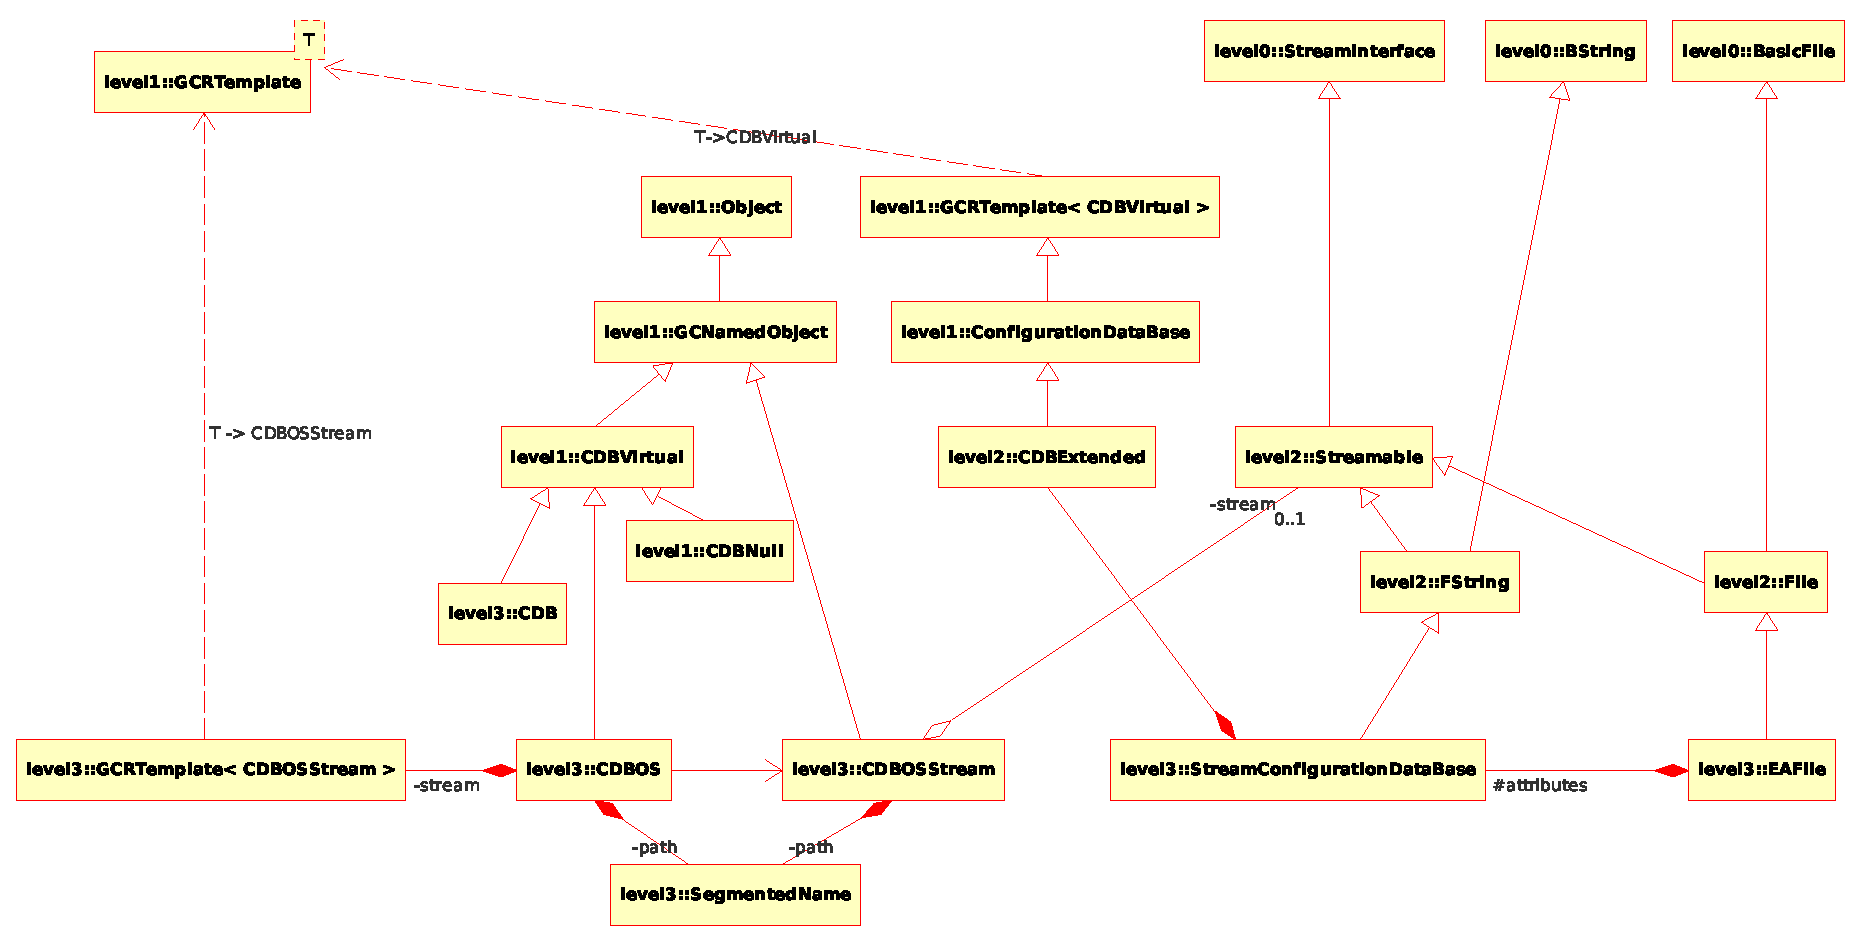
\includegraphics[width=\textwidth]{level3/level3-otherCDB.eps}
  \caption{BaseLib Level3 CDBOS and SCDB}
  \label{f:level3:otherCDB}
 \end{center}
\end{figure}



\subsection{CDBOS}
TODO\\
TODO\\
TODO\\
CHE COSA E e cosa fa

\begin{figure}[h!]
 \begin{center}
  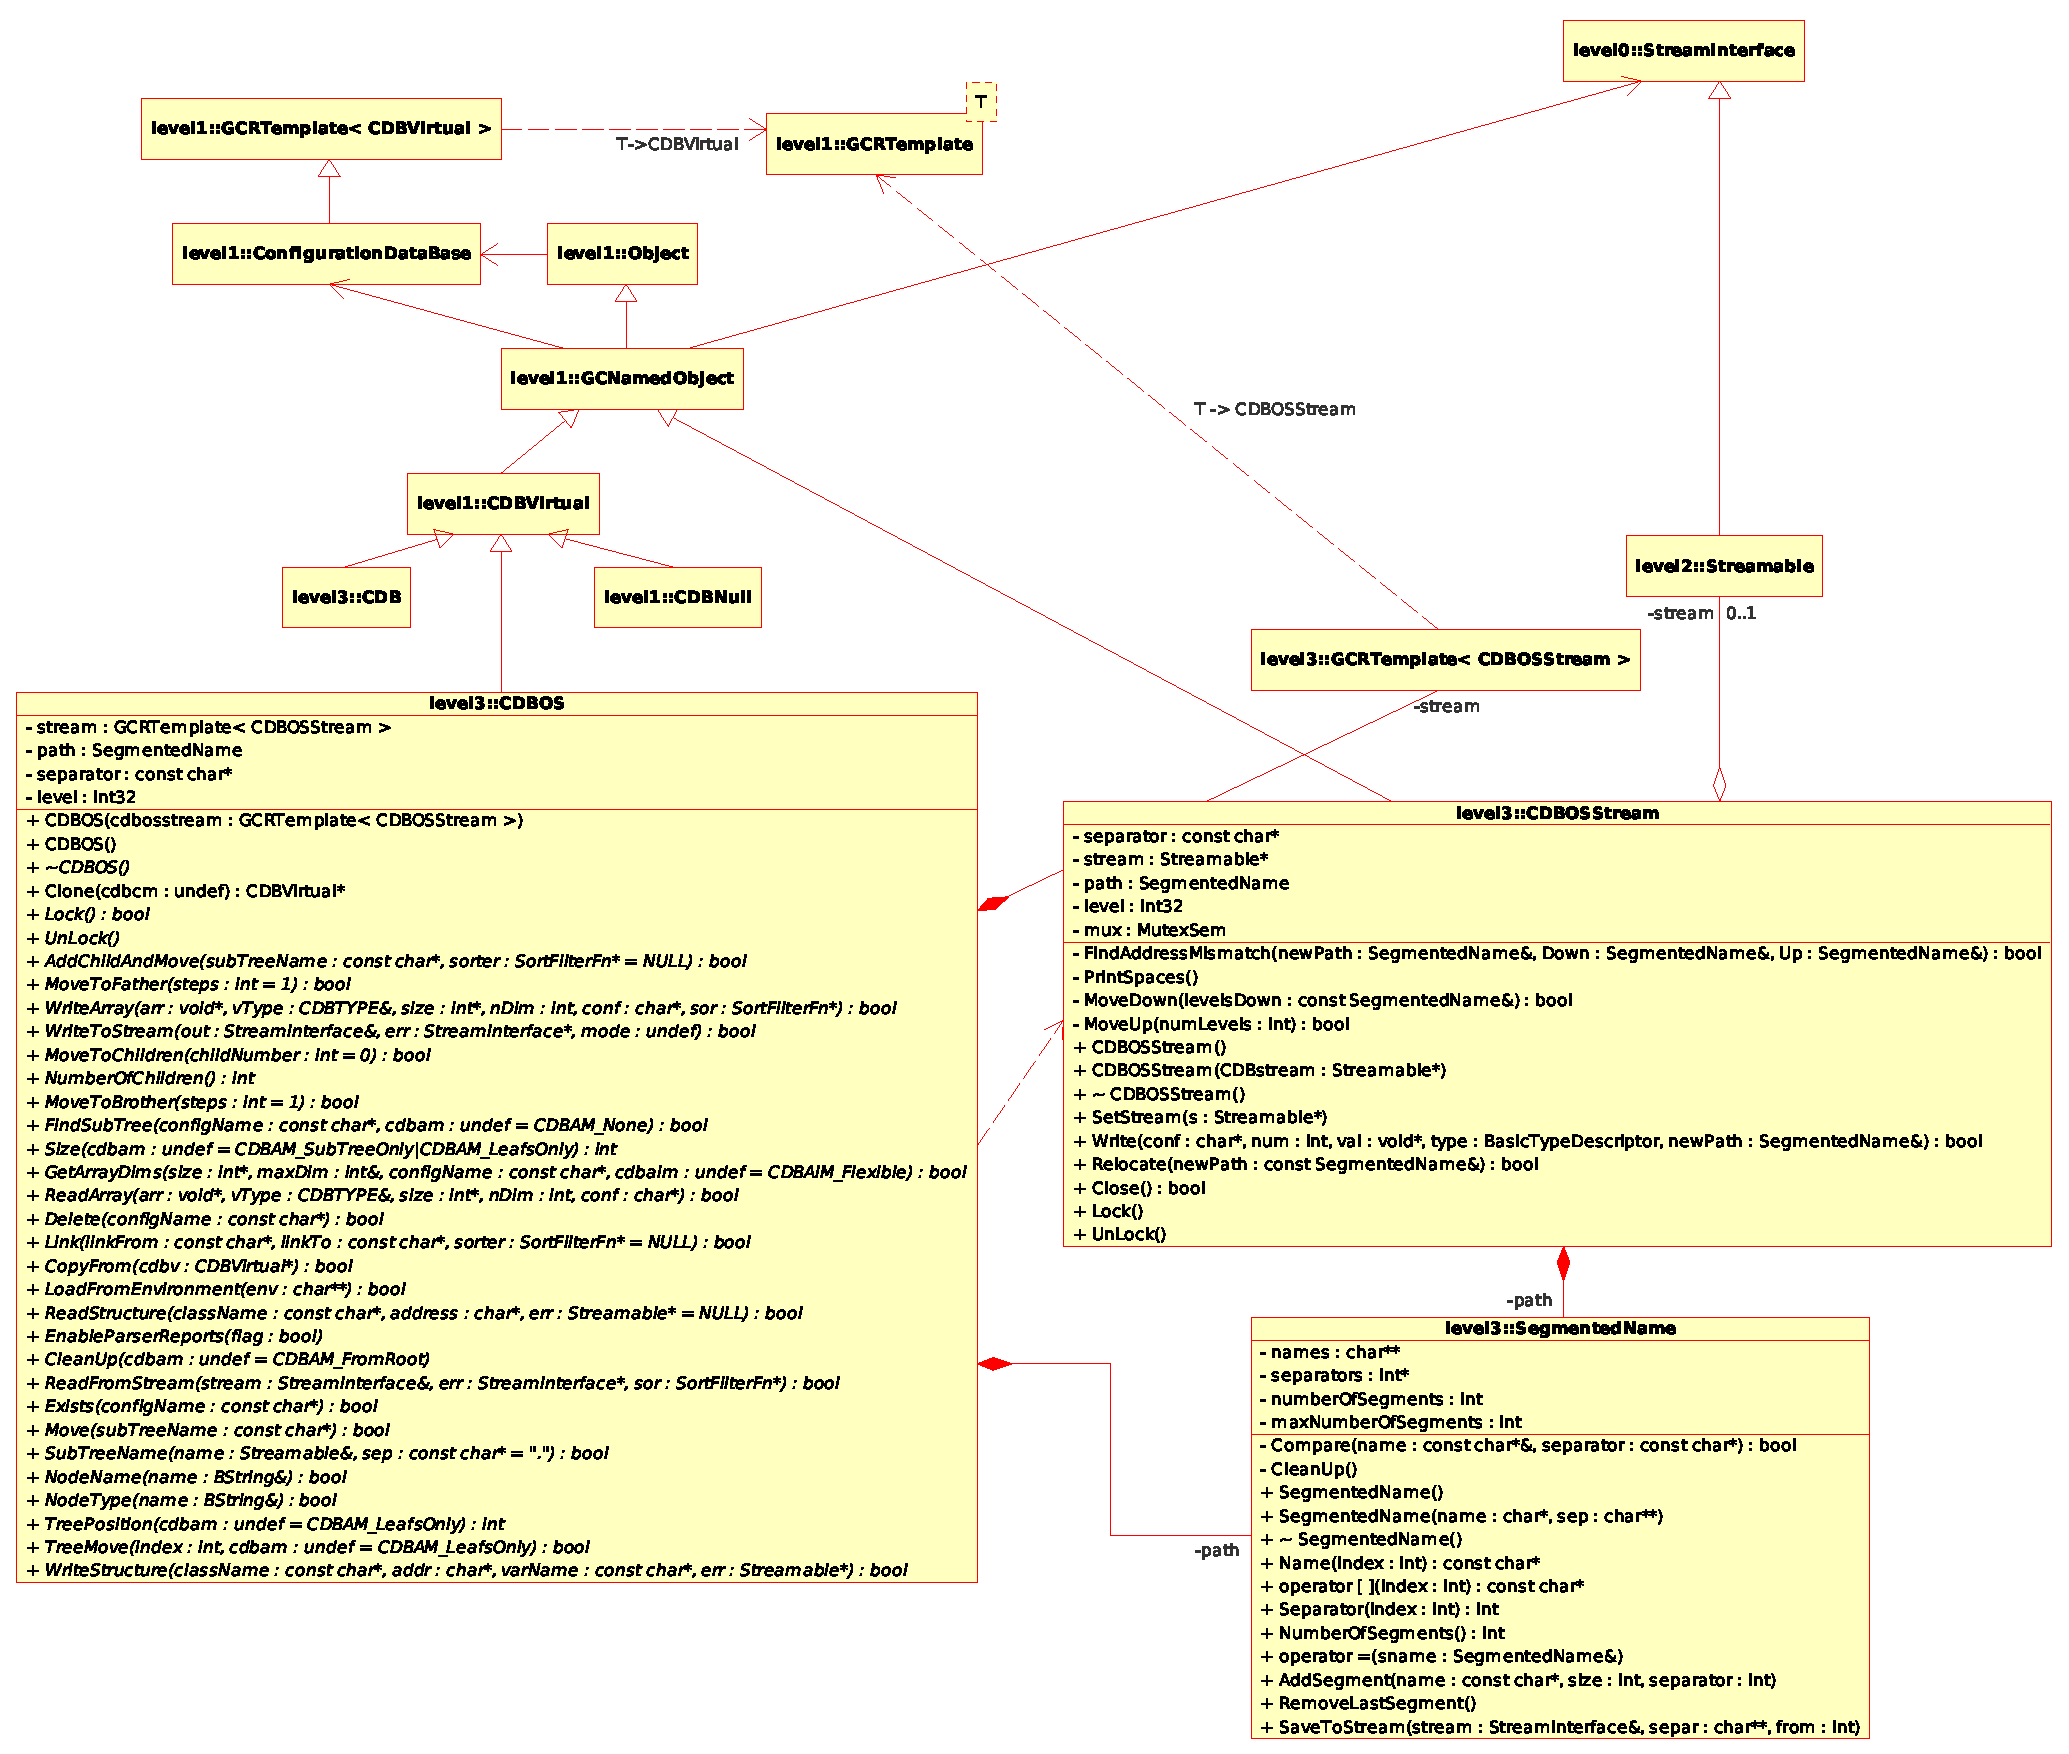
\includegraphics[width=\textwidth]{level3/level3-CDBOS.eps}
  \caption{BaseLib Level3 CDBOS (another Configuration Database implementation)}
  \label{f:level3:CDBOS}
 \end{center}
\end{figure}


\begin{itemize}
 \item SegmentedName
 \item CDBOSStream
 \item CDBOS
\end{itemize}



\subsubsection{SegmentedName}
\texttt{[SegmentedName.h]}\\
The class \texttt{SegmentedName} doesn't inherit from any other class. Such class parses a name with segments like paths or structure naming. For example it can be used to segment a UNIX path like this:

\begin{lstlisting}[
extendedchars=true,%
basicstyle=\fontfamily{pcr}\fontseries{m}\selectfont\footnotesize, %
stepnumber=1,%
numberstyle=\tiny,%
keywordstyle=\footnotesize\tt ,%
language=bash]
/usr/include/asm-generic/bitops/atomic.h
\end{lstlisting}

in two data structures: an array of character strings, the segments (attribute \texttt{names} see below the source), and an array of index of separators (attribute \texttt{separators}). The parsing of the path above load the class with the following contents:
\begin{table}[!h]
 \begin{center}
  \begin{tabular}{|c|c|c|}
   \hline
index & \texttt{char** names} & \texttt{int* separators} \\
    \hline
0 & usr & \texttt{/} \\
1 & include & \texttt{/} \\
2 & asm-generic & \texttt{/} \\
3 & bitops & \texttt{/} \\
4 & atomic & \texttt{/} \\
5 & h & \texttt{.} \\
    \hline
    \end{tabular}
   \end{center}
  \caption{Level3 \texttt{SegmentedName} class attributes}
 \label{t:level3:SegmentedName}
\end{table}

From the source we know the four attribtues on which the class is build up, the first attribute, \texttt{names} is a zero separated names array, \texttt{separators} is an index in the separators list provided at object construction (note that in the attribute list there is no such list). \texttt{numberOfSegments} is the current number of segments added to the list, \texttt{maxNumberOfSegments} is the actually max number of segments in the class.
\begin{lstlisting}[
extendedchars=true,%
basicstyle=\fontfamily{pcr}\fontseries{m}\selectfont\footnotesize, %
stepnumber=1,%
numberstyle=\tiny,%
keywordstyle=\footnotesize\tt ,%
language=C++]
private:
   char** names;
   int* separators;
   int numberOfSegments;
   int maxNumberOfSegments;
\end{lstlisting}

The method \texttt{Compare} is similar to the well known \texttt{strcmp} but limit search to size of separators, \texttt{CleanUp} simply free all associated structures (char strings) of a class.

Teh first constructor create a new \texttt{null} \texttt{SegmenetedName}, the second one take as arguments a character string containing a name to be segmented and a separators list, i.e. a \texttt{NULL} terminated vector of separators strings. \\


The method \texttt{Name} returns the \texttt{index}-th segment, \texttt{Separator} returns the index of the \texttt{index}-th separator in the string. \texttt{NumberOfSegments} returns the currently available segments in the class. Then two operator ridefinition are coming. \texttt{AddSegment} simply let you to add a segment manually, that you can remove with \texttt{RemoveLastSegment}. With the method \texttt{SaveToStream} it is possible to recompone the segmented name saved starting from any segment (see \texttt{fromSegment} argument).
\begin{lstlisting}[
extendedchars=true,%
basicstyle=\fontfamily{pcr}\fontseries{m}\selectfont\footnotesize, %
stepnumber=1,%
numberstyle=\tiny,%
keywordstyle=\footnotesize\tt ,%
language=C++]
   bool Compare(const char*& name,const char* separator);
   void CleanUp();

public:
   SegmentedName();
   SegmentedName(const char* name,const char** separatorNames);
   ~SegmentedName();

   const char* Name(int index) const;
   int Separator(int index);
   int NumberOfSegments() const;
   const char* operator[](int index) const;
   void operator=(SegmentedName& sname);

   void AddSegment(const char* name,int size,int separator);
   void RemoveLastSegment();
   void SaveToStream(StreamInterface& stream,const char** separatorNames=NULL,
      int fromSegment=0);
\end{lstlisting}



\subsubsection{CDBOSStream}
\texttt{[CDBOSStream.h]}\\
The class \texttt{CDBOSStream} is used from the class \texttt{CDBOS}, so it is presented before. \\


The first attribute is a character string \texttt{separator} that holds a list of separator, single character separators. The second attribute is a pointer to a \texttt{Streamable}, i.e. an interal pointer to the \texttt{Streamable} to write the \texttt{CDB} content. The attribute \texttt{path} is a \texttt{SegmentedName} that holds the current path in the CDB, \texttt{level} stores the current level in the hierarchy and the \texttt{MutexSem} protects against concurrent operations on the data structure.

\begin{lstlisting}[
extendedchars=true,%
basicstyle=\fontfamily{pcr}\fontseries{m}\selectfont\footnotesize, %
stepnumber=1,%
numberstyle=\tiny,%
keywordstyle=\footnotesize\tt ,%
language=C++]
private:
   const char* separator;
   Streamable* stream;
   SegmentedName path;
   int32 level;
   MutexSem mux;
\end{lstlisting}

We take a look at the methods of the class; method \texttt{FindAddressMismatch} finds differences between two \texttt{CDB} addresses; \texttt{PrintSpaces} prints spaces to respect hierarchy, \texttt{MoveDown} moves \textbf{n} levels down the structure and \texttt{MoveUp} moves \textbf{n} levels up the structure. \\


The constructor initialize the class by default with separator \texttt{``/''}. The method \texttt{SetStream} sets the \texttt{stream} attribute; \texttt{Write} writs to the output one value at the current address.
\texttt{Relocate} lets move in the CDB and update internal path; \texttt{Close} closes the parenthesis opened untill now; methods \texttt{Lock} and \texttt{UnLock} locks and unlock the stream's semaphore.
\begin{lstlisting}[
extendedchars=true,%
basicstyle=\fontfamily{pcr}\fontseries{m}\selectfont\footnotesize, %
stepnumber=1,%
numberstyle=\tiny,%
keywordstyle=\footnotesize\tt ,%
language=C++]
   bool FindAddressMismatch(const SegmentedName& newPath,int& levelsUp,
      SegmentedName& levelsDown);
   void PrintSpaces();
   bool MoveDown(const SegmentedName& levelsDown);
   bool MoveUp int numLevels);

public:
   CDBOSStream(): separator("/"), path("",&separator);
   CDBOSStream(Streamable* CDBstream) : separator("/"),path("",&separator);
   ~CDBOSStream();

   void SetStream(Streamable* s);
   bool Write (const char* configName,int numOfElements,const void* value,
      BasicTypeDescriptor type,const SegmentedName& newPath);

   bool Relocate (const SegmentedName& newPath);
   bool Close();
   void Lock();
   void UnLock();
\end{lstlisting}

The class \texttt{CDBOSStream} is used to templatize a \texttt{GCRTemplate} that is then used as an attribute in the following \texttt{CDBOS} class.



\subsubsection{CDBOS}
\texttt{[CDBOS.h, CDBOS.cpp]}\\
The class \texttt{CDBOS} inherits from \texttt{CDBVirtual}, the \texttt{CDBOS} implement direct writing of a \textit{Configuration Database} to a stream. The first attribute is a \texttt{GCRTemplate< CDBOSStream >}, i.e. an object that has a pointer to a \texttt{CDBOSStream}. The attribute \texttt{path} save the current path inside the \texttt{CDB}, \texttt{separator} is a character array of separators and \texttt{level} stores the current level in the hierarchy in the same way as they do in the \texttt{CDBOSStream} class.
\begin{lstlisting}[
extendedchars=true,%
basicstyle=\fontfamily{pcr}\fontseries{m}\selectfont\footnotesize, %
stepnumber=1,%
numberstyle=\tiny,%
keywordstyle=\footnotesize\tt ,%
language=C++]
private:
   GCRTemplate<CDBOSStream> stream;
   SegmentedName path;
   const char* separator;
   int32 level;

   CDBOS(GCRTemplate<CDBOSStream> cdbosstream) : separator("/"), path("",&separator);
   CDBOS() : stream(GCFT_Create), separator("/"), path("",&separator);
   virtual ~CDBOS();
\end{lstlisting}

The method \texttt{Clone} returns a \texttt{CDBVirtual} pointer creating a new reference to a database, or if that is not possible it creates a copy of it; if \texttt{cdbcm} is \texttt{CDBCM\_CopyAddress} ensures that the new object points at the same location.

The method \texttt{Lock} locks the main database for exclusive access: use if a group of transactions should be atomic; \texttt{UnLock} unlocks the main database: remember to unlock a locked database after using it.

The method \texttt{AddChilAndMove} can be used to create a new subtree, \texttt{MoveToFather} move the current pointer to the father's node, $-1$ means moving to the root node. \\


The method \texttt{WriteArray} calls the method \texttt{GCRTemplate< CDBOSStream >::Write}, if \texttt{size} is \texttt{NULL} it treats the input as a monodimensional array of size \texttt{nDim}. The method \texttt{WriteToStream} is used to write to the stream assigned.
\begin{lstlisting}[
extendedchars=true,%
basicstyle=\fontfamily{pcr}\fontseries{m}\selectfont\footnotesize, %
stepnumber=1,%
numberstyle=\tiny,%
keywordstyle=\footnotesize\tt ,%
language=C++]
public:
   CDBVirtual* Clone(CDBCreationMode cdbcm);
   virtual bool Lock();
   virtual void UnLock();

   virtual bool AddChildAndMove(const char* subTreeName,SortFilterFn* sorter=NULL);
   virtual bool MoveToFather(int steps=1);

   virtual bool WriteArray(const void* array,const CDBTYPE& valueType,const int* size,
      int nDim,const char* configName,SortFilterFn* sorter=NULL);
   virtual bool WriteToStream(StreamInterface& streamout,StreamInterface* err=NULL,
      CDBWriteMode mode=CDBWM_Tree);
\end{lstlisting}

Then follow a huge list of overridden methods that simply returns an error because are not implemented in this class.

\begin{lstlisting}[
extendedchars=true,%
basicstyle=\fontfamily{pcr}\fontseries{m}\selectfont\footnotesize, %
stepnumber=1,%
numberstyle=\tiny,%
keywordstyle=\footnotesize\tt ,%
language=C++]
    virtual bool MoveToChildren(int childNumber=0);
    virtual int  NumberOfChildren();
    virtual bool MoveToBrother(int steps=1);
    virtual bool FindSubTree(const char* configName,CDBAddressMode cdbam=CDBAM_None);
    virtual int  Size(CDBAddressMode cdbam=CDBAM_SubTreeOnly | CDBAM_LeafsOnly)
    virtual bool GetArrayDims(int* size,int& maxDim,const char* configName,CDBArrayIndexingMode cdbaim=CDBAIM_Flexible);
    virtual bool ReadArray(void* array,const CDBTYPE& valueType,const int* size,int nDim,const char* configName);
    virtual bool Delete(const char* configName);
    virtual bool Link(const char* linkFrom,const char* linkTo,SortFilterFn* sorter=NULL);
    virtual bool CopyFrom(CDBVirtual* cdbv);
    virtual bool LoadFromEnvironment(char** env);
    virtual bool ReadStructure (const char* className,char* address,Streamable* err=NULL);
    virtual void EnableParserReports(bool flag);
    virtual void CleanUp(CDBAddressMode cdbam=CDBAM_FromRoot);
    virtual bool ReadFromStream(StreamInterface& stream,StreamInterface* err=NULL,SortFilterFn* sorter=NULL);
    virtual bool Exists(const char* configName);
    virtual bool Move(const char* subTreeName);
    virtual bool SubTreeName(Streamable& name,const char* sep = ".")
    virtual bool NodeName(BString& name);
    virtual bool NodeType(BString& name);
    virtual int  TreePosition(CDBAddressMode cdbam=CDBAM_LeafsOnly);
    virtual bool TreeMove(int index,CDBAddressMode cdbam=CDBAM_LeafsOnly);
    virtual bool WriteStructure(const char* className,char* address,const char* variableName=NULL,Streamable* err=NULL);
\end{lstlisting}



\subsection{Stream Configuration Database (SCDB)}
The \textit{Stream Configuration Database} is another kind of \textit{Configuration Database} that is really similar to the \texttt{CDBOS} structure.
Figure \ref{f:level3:SCDB} represent the UML schema of the \textit{Stream Configuration Database} infrastructure.
Classes in this section are:
\begin{itemize}
 \item StreamConfigurationDataBase
 \item EAFile
\end{itemize}
The \texttt{EAFile} is grouped in this section because it is the only user of the SCDB in this section.
\begin{figure}[h!]
 \begin{center}
  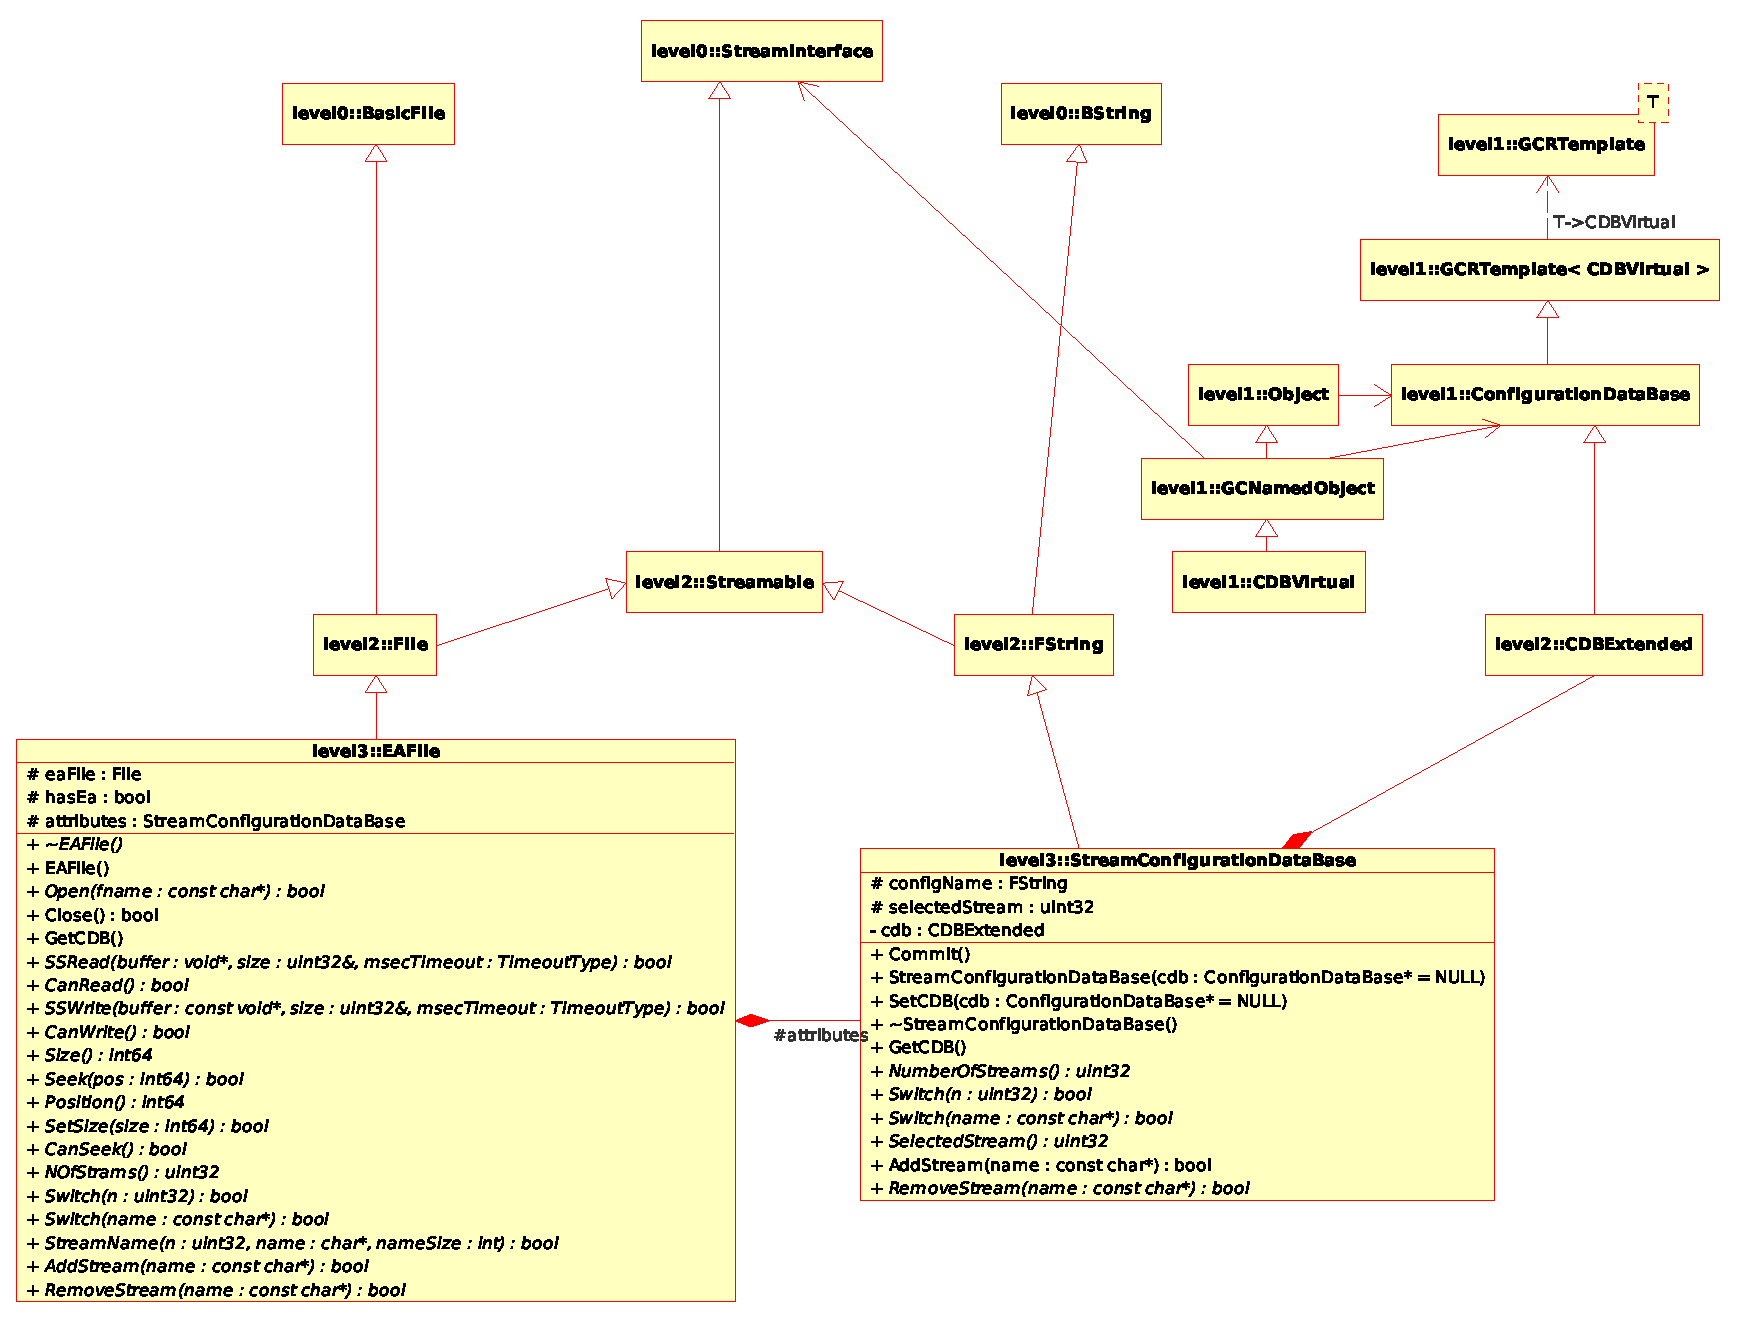
\includegraphics[width=\textwidth]{level3/level3-SCDB.eps}
  \caption{BaseLib Level3 SCDB (another Configuration Database implementation)}
  \label{f:level3:SCDB}
 \end{center}
\end{figure}



\subsubsection{StreamConfigurationDataBase}
\texttt{[StreamConfigurationDataBase.h, StreamConfigurationDataBase.cpp]}\\
The class \texttt{StreamConfigurationDataBase} implement a \textit{Configuration Database} using the multi stream interface to read and write data into, so it is far different from the \texttt{CDBOS} because is a \texttt{Streamable}, more precisely a \texttt{FString}, that has a \texttt{CDBExtended} as an attribute. With a SCDB it is possible to write and read to a CDB like a stream. \\


The first attribute \texttt{cdb} is the \texttt{CDBExtended} associated to the SCDB, i.e. the CDB being modified; \texttt{configName} is the current location pointer and \texttt{selectedStream} is the order of current location within tree.
\begin{lstlisting}[
extendedchars=true,%
basicstyle=\fontfamily{pcr}\fontseries{m}\selectfont\footnotesize, %
stepnumber=1,%
numberstyle=\tiny,%
keywordstyle=\footnotesize\tt ,%
language=C++]
protected:
   CDBExtended cdb;
   FString configName;
   uint32 selectedStream;
\end{lstlisting}

The method \texttt{Commit} copies the work done to the stream this far to the database, the constructor initialises with a reference to a \textit{CDB} the destructor basically calls \texttt{Commit} and \texttt{SetCDB} like the constructor initialises with a reference \textit{CDB}; \texttt{GetCDB} gets the \texttt{cdb} attribute. \\


The method \texttt{NumberOfStreams} returns how many streams are available in total, counts from root all the leaves. \texttt{SelectedStream} returns which is the selected stream. Methods \texttt{Switch} select the stream to read from, switching may reset the stream to the start. The method \texttt{AddStream} adds a new stream to write to and \texttt{RemoveStream} removes an existing stream.
\begin{lstlisting}[
extendedchars=true,%
basicstyle=\fontfamily{pcr}\fontseries{m}\selectfont\footnotesize, %
stepnumber=1,%
numberstyle=\tiny,%
keywordstyle=\footnotesize\tt ,%
language=C++]
public:
   void Commit();

   StreamConfigurationDataBase(ConfigurationDataBase* cdb = NULL):cdb("CDB");
   ~StreamConfigurationDataBase();

   void SetCDB(ConfigurationDataBase* cdb = NULL);
   CDBExtended& GetCDB();

   virtual uint32 NumberOfStreams();
   virtual uint32 SelectedStream();
   virtual bool Switch(uint32 n);
   virtual bool Switch(const char *name);

   bool AddStream(const char *name);
   virtual bool RemoveStream(const char *name){
\end{lstlisting}



\subsubsection{EAFile}
\texttt{[EAFile.h, EAFile.cpp]}\\
The class \texttt{EAFile} stands for \textit{Extended Attributes File}, it accounts to store extended attributes of files that a File Systema of an OS doesn't account for in a separate file; such files have the following extension, we paste the definition below.
\begin{lstlisting}[
extendedchars=true,%
basicstyle=\fontfamily{pcr}\fontseries{m}\selectfont\footnotesize, %
stepnumber=1,%
numberstyle=\tiny,%
keywordstyle=\footnotesize\tt ,%
language=C++]
#define EA_EXT ".!EA!"
\end{lstlisting}

The class inherits from \texttt{File} so its a \texttt{Streamable}. The first atrribute, \texttt{eaFile} is a \texttt{File} so it not only inherits from \texttt{File} but has also an attribute of the same type, and such attribute refers to the file containing the attributes. \texttt{hasEa} is \texttt{true} if any attributes have been set; \texttt{attributes} is a stream interface to the attributes.
\begin{lstlisting}[
extendedchars=true,%
basicstyle=\fontfamily{pcr}\fontseries{m}\selectfont\footnotesize, %
stepnumber=1,%
numberstyle=\tiny,%
keywordstyle=\footnotesize\tt ,%
language=C++]
protected:
   File eaFile;
   bool hasEa;
   StreamConfigurationDataBase attributes;
\end{lstlisting}

We skip destructor and constructor because are without arguments. The \texttt{Open} method opens for read/write or create if missing the \textit{Extended Attribute File}, \texttt{Close} closes it. \texttt{GetCDB} get the \texttt{attribute} attribute content. All other methos are from the \texttt{Streamable} interface. \\


The method \texttt{SSRead} reads from the selected stream, \texttt{SSWrite} writes to the selected stream, methods \texttt{CanRead} and \texttt{CanWrite} return the capability of reading and writing of the \texttt{attribute}.
\begin{lstlisting}[
extendedchars=true,%
basicstyle=\fontfamily{pcr}\fontseries{m}\selectfont\footnotesize, %
stepnumber=1,%
numberstyle=\tiny,%
keywordstyle=\footnotesize\tt ,%
language=C++]
public:
   virtual ~EAFile();
   EAFile()

   virtual bool Open(const char *fname,...);
   bool Close();

   CDBExtended& GetCDB();

   virtual bool SSRead (void* buffer,uint32& size,TimeoutType msecTimeout);
   virtual bool CanRead();
   virtual bool SSWrite(const void* buffer,uint32& size,TimeoutType msecTimeout);
   virtual bool CanWrite();
\end{lstlisting}

The method \texttt{Size} returns the size of the file; \texttt{SetSize} clips the file size to a specified point; \texttt{Position} returns the current position in the file; \texttt{Seek} moves within the file to an absolute location, \texttt{CanSeek} return \texttt{true} if seeking is possible. \\


The method \texttt{NOfStreams} gets how many streams are available; methods \texttt{Switch} select the stream to read from, switching may reset the stream to the start. \texttt{StreamName} returns the name of the stream \texttt{n}, stream \texttt{0} is the file and therefore you get the file name. \texttt{AddStream} adds a new stream to write to, \texttt{selectedStream} is resetted to \texttt{0}; \texttt{RemoveStream} removes a stream.
\begin{lstlisting}[
extendedchars=true,%
basicstyle=\fontfamily{pcr}\fontseries{m}\selectfont\footnotesize, %
stepnumber=1,%
numberstyle=\tiny,%
keywordstyle=\footnotesize\tt ,%
language=C++]
   virtual int64 Size();
   virtual bool SetSize(int64 size);
   virtual int64 Position(void);
   virtual bool Seek(int64 pos);
   virtual bool CanSeek();

   virtual uint32 NOfStreams();
   virtual bool Switch(uint32 n);
   virtual bool Switch(const char* name);
   virtual bool StreamName(uint32 n,char* name,int nameSize);
   virtual bool AddStream(const char* name);
   virtual bool RemoveStream(const char* name)
\end{lstlisting}



\subsection{Design Notes}
The class \texttt{SegmentedName} supports separators of only one character. How it is possible to handle separators made up of one or more characters, i.e. how it is possible to handle an URL like
\begin{lstlisting}[
extendedchars=true,%
basicstyle=\fontfamily{pcr}\fontseries{m}\selectfont\footnotesize, %
stepnumber=1,%
numberstyle=\tiny,%
keywordstyle=\footnotesize\tt ,%
language=bash]
http://www.google.it
\end{lstlisting}


\section{Parser}
The following classes address the problem of parsing a string, all classes create a framework to build up a parser.
In Figure \ref{f:level3:parser} is depicted the UML schema of the parser infrastructure.
The following classes are involved:
\begin{itemize}
 \item LA\_TokenInfo
 \item LA\_TokenData
 \item LexicalAnalyzer
 \item Parser
\end{itemize}

\begin{figure}[h!]
 \begin{center}
  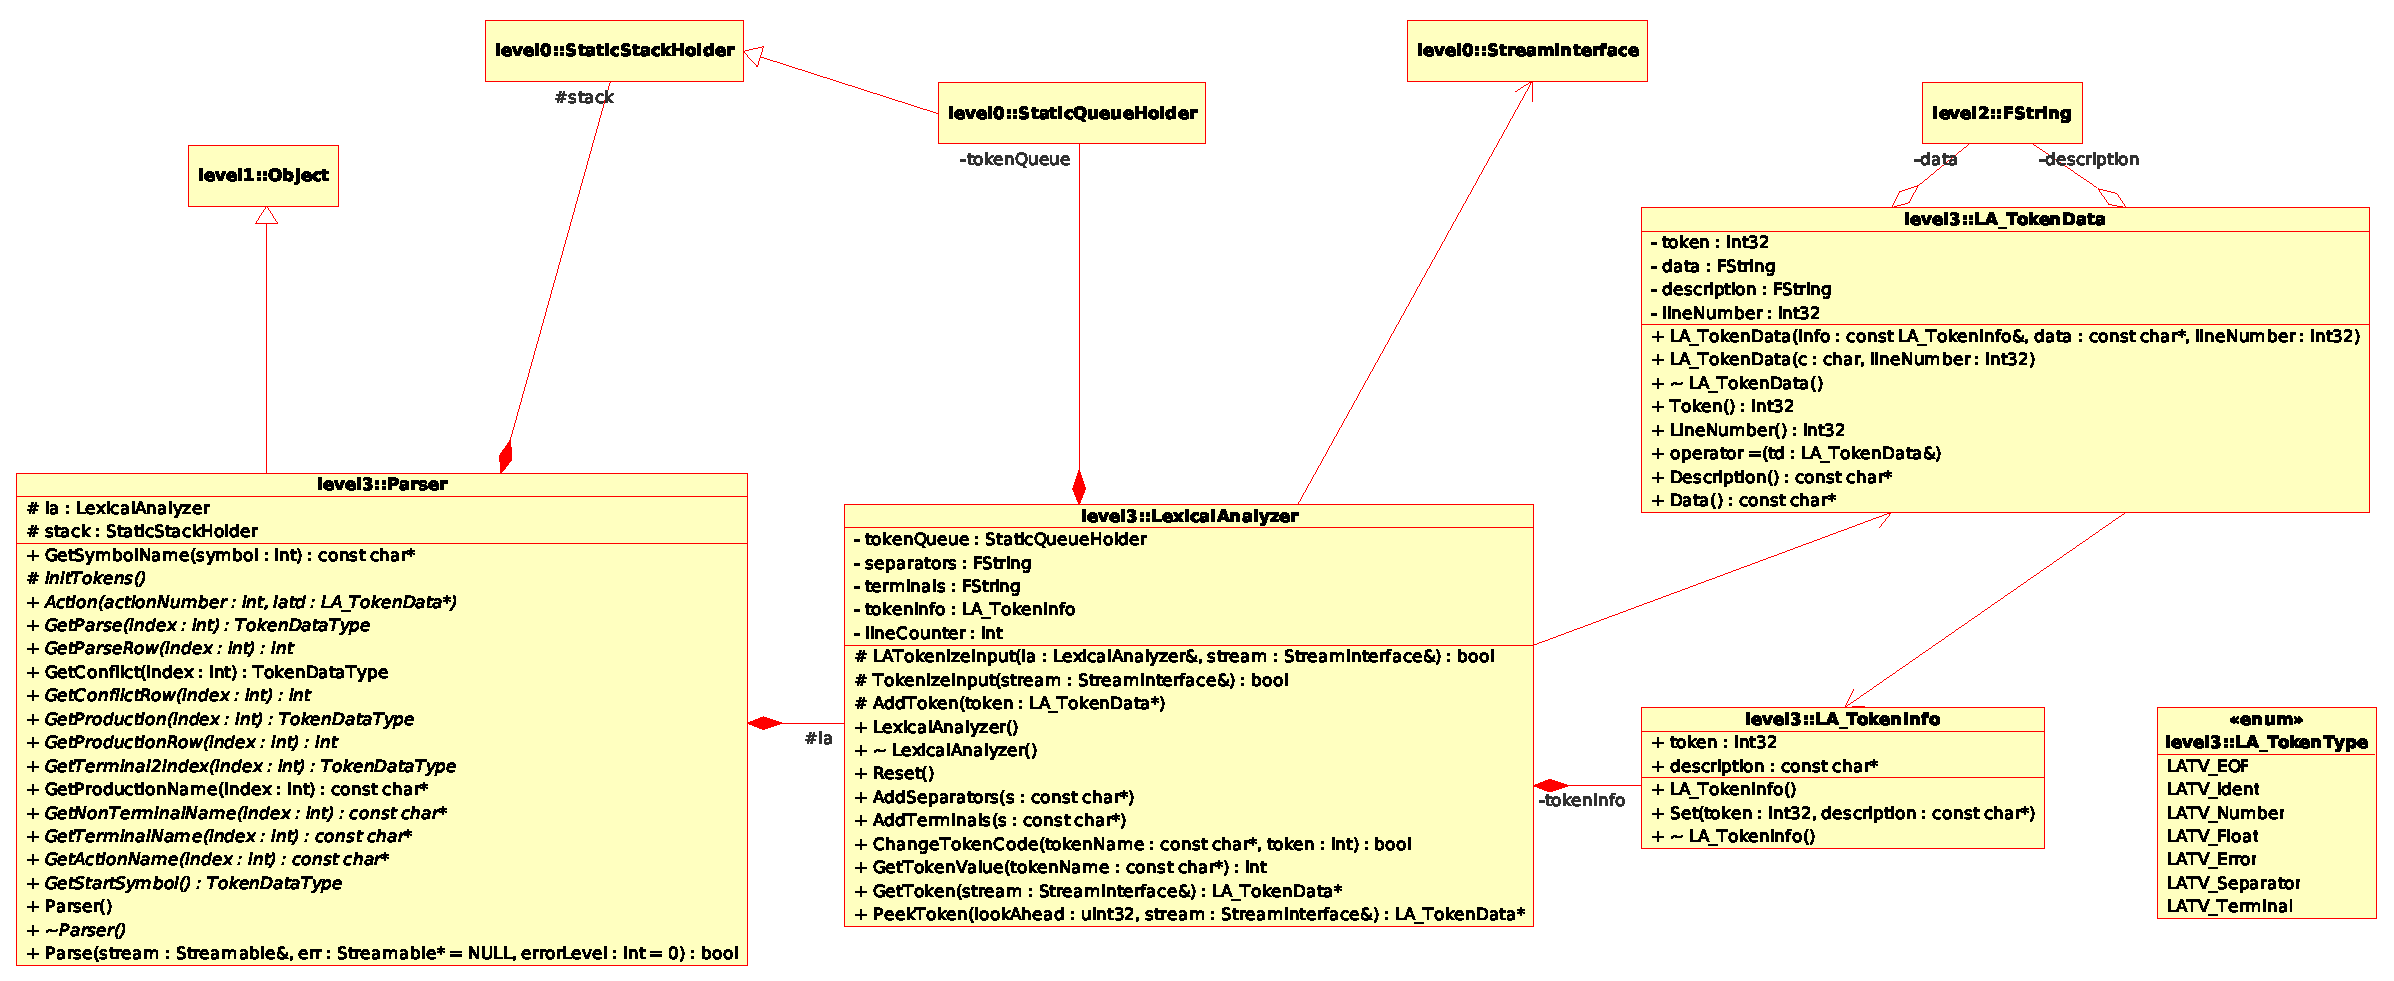
\includegraphics[width=\textwidth]{level3/level3-parser.eps}
  \caption{BaseLib Level3 parser, lexical analyser and tokenizer}
  \label{f:level3:parser}
 \end{center}
\end{figure}



\subsubsection{Lexical Analyzer Token Information}
\texttt{[LexicalAnalyzer.h, LexicalAnalyzer.cpp]}\\
The class \texttt{LA\_TokenInfo} stores information about a lexical element. The first attribute, \texttt{token} is the code identifying the lexical meaning of this part of the text, \texttt{description} holds the meaning of the token.
The constructor initialize \texttt{token} to zero and \texttt{description} to \texttt{NULL}, the method \texttt{Set} lets you setting the attributes.
\begin{lstlisting}[
extendedchars=true,%
basicstyle=\fontfamily{pcr}\fontseries{m}\selectfont\footnotesize, %
stepnumber=1,%
numberstyle=\tiny,%
keywordstyle=\footnotesize\tt ,%
language=C++]
public:
   int32 token;
   const char* description;

   LA_TokenInfo();
   ~LA_TokenInfo();
   void Set(int32 token,const char* description);
\end{lstlisting}



\subsubsection{Lexical Analyzer Token Data}
\texttt{[LexicalAnalyzer.h, LexicalAnalyzer.cpp]}\\
The class \texttt{LA\_TokenData} is an element produced by the \texttt{LexicalAnalyzer}. The attribute \texttt{token} is the code identifying the lexical meaning of this part of the text; \texttt{data} is the parsed part of the text; \texttt{description} is copied from a \texttt{LA\_TokenInfo}, it holds the meaning of the token; \texttt{lineNumber} saves at what line the token was found.
\begin{lstlisting}[
extendedchars=true,%
basicstyle=\fontfamily{pcr}\fontseries{m}\selectfont\footnotesize, %
stepnumber=1,%
numberstyle=\tiny,%
keywordstyle=\footnotesize\tt ,%
language=C++]
   int32 token;
   FString data;
   FString description;
   int32 lineNumber;
\end{lstlisting}

The first constructor builds a token from a token description constant and the data content, the second constructor builds a token from a simple character.

The method \texttt{Token} returns the attribute \texttt{token}; \texttt{LineNumber} returns the attribute \texttt{lineNumber}; the \texttt{operator=} redefinition copies content, \texttt{Description} return the description of the content and \texttt{Data} return the content, i.e. \texttt{data} attribute.
\begin{lstlisting}[
extendedchars=true,%
basicstyle=\fontfamily{pcr}\fontseries{m}\selectfont\footnotesize, %
stepnumber=1,%
numberstyle=\tiny,%
keywordstyle=\footnotesize\tt ,%
language=C++]
public:
   LA_TokenData(const LA_TokenInfo &info, const char *data,int32 lineNumber);
   LA_TokenData(char c,int32 lineNumber);
   virtual ~LA_TokenData();

   int32 Token();
   int32 LineNumber();
   void  operator=(LA_TokenData& td);
   const char* Description();
   const char* Data();
\end{lstlisting}



\subsubsection{Lexical Analyzer}
\texttt{[LexicalAnalyzer.h, LexicalAnalyzer.cpp]}\\
The class \texttt{LexicalAnalyzer} is a slightly programmable lexical analyzer; It recognizes \textit{identifiers}, \textit{numbers} and \textit{floats}. It allows to browse ahead without consuming the token, tokenisation is performed on demand.\\


Before exploring the class we paste an enumeration below. This enumeration is a set of codes to list the complex terminals recognised by the analyser. The source code is self explained.
\begin{lstlisting}[
extendedchars=true,%
basicstyle=\fontfamily{pcr}\fontseries{m}\selectfont\footnotesize, %
stepnumber=1,%
numberstyle=\tiny,%
keywordstyle=\footnotesize\tt ,%
language=C++]
enum LA_TokenType{
   /** indicates EOF */
   LATV_EOF=0x100,
   /** indicates an identifier or a string */
   LATV_Ident=0x101,
   /** indicates an integer */
   LATV_Number=0x102,
   /** indicates a float */
   LATV_Float=0x103,
   /** indicates a wrongly constructed element */
   LATV_Error=0x104,
   /** indicates an element that separates parts of the phrase */
   LATV_Separator=0x105,
   /** indicates an element that is a token on its own */
   LATV_Terminal=0x106
};
\end{lstlisting}

The first attribute, \texttt{tokenQueue} is a queue of pre-cooked tokens; \texttt{separators} is a string made of separators; \texttt{terminals} is a string composed of the terminal characters; \texttt{tokenInfo} list of token informations.
\begin{lstlisting}[
extendedchars=true,%
basicstyle=\fontfamily{pcr}\fontseries{m}\selectfont\footnotesize, %
stepnumber=1,%
numberstyle=\tiny,%
keywordstyle=\footnotesize\tt ,%
language=C++]
   StaticQueueHolder tokenQueue;
   FString separators;
   FString terminals;
   LA_TokenInfo tokenInfo[LATV_Error+2-0x100];
   int lineCounter;
\end{lstlisting}

The method \texttt{TokenizeInput} is the main method that takes as an argument a \texttt{StreamInterface} and with the \texttt{this} pointer calls a friend C method \texttt{LA\_TokenizeInput} that make the tokenization of the input stream; every token is also added to the \texttt{tokenQueue}.

The method \texttt{AddToken} adds a token into the \texttt{tokenQueue}. \texttt{Reset} resets the status of the class; \texttt{AddSeparators} sets these characters as separators; \texttt{AddTerminals} sets these characters as separators; \texttt{ChangeTokenCode} changes the token code associated with a given complex terminal, valid \texttt{tokenNames} are:
\begin{itemize}
 \item "EOF"
 \item "IDENT"
 \item "NUMBER"
 \item "FLOAT"
 \item "ERROR"
\end{itemize}

The method \texttt{GetToken} takes one token from the stack or processes the input for a new one, moves the token into last token. The class allocates the data but does not provide to the deallocation once the structure has been extracted.
The method \texttt{PeekToken} reads in the stack at position \texttt{lookAhead} argument or increases the stack to allow for it; it returns the token but it still keeps hold of it.

\begin{lstlisting}[
extendedchars=true,%
basicstyle=\fontfamily{pcr}\fontseries{m}\selectfont\footnotesize, %
stepnumber=1,%
numberstyle=\tiny,%
keywordstyle=\footnotesize\tt ,%
language=C++]
protected:
   bool TokenizeInput(StreamInterface &stream);
   void AddToken(LA_TokenData* token);

public:
   LexicalAnalyzer(): tokenQueue(sizeof(LA_TokenData*)/sizeof(int));
   ~LexicalAnalyzer()

   void Reset();
   void AddSeparators(const char* s);
   void AddTerminals(const char* s);
   bool ChangeTokenCode(const char* tokenName,int token);

   int GetTokenValue(const char* tokenName);

   LA_TokenData* GetToken(StreamInterface& stream);
   LA_TokenData* PeekToken(uint32 lookAhead,StreamInterface& stream);
\end{lstlisting}



\subsubsection{Parser}
\texttt{[Parser.h, Parser.cpp]}\\
The class \texttt{Parser} allows implementation of parsers. It is a base class for parsers. The class inherits from \texttt{Object}. The first attribute, of type \texttt{LexicalAnalyzer}, is the lexical analyzer; second attribute is a \texttt{StaticStackHolder}. \\


The method \texttt{GetSymbolName} gets the symbol name from an index. The method \texttt{Parse} 
parses a \texttt{Streamable} passed by argument, \texttt{errorLevel} can be one of the following:
\begin{itemize}
 \item \texttt{0} means do not display
 \item \texttt{1} means show actions
 \item \texttt{2} means show productions
 \item \texttt{-1} means show all
\end{itemize}

\begin{lstlisting}[
extendedchars=true,%
basicstyle=\fontfamily{pcr}\fontseries{m}\selectfont\footnotesize, %
stepnumber=1,%
numberstyle=\tiny,%
keywordstyle=\footnotesize\tt ,%
language=C++]
protected:
   LexicalAnalyzer la;
   StaticStackHolder stack;
private:
   const char* GetSymbolName(int symbol);
public:
   Parser():stack(sizeof(TokenDataType)/sizeof(int));
   virtual ~Parser();
   bool Parse(Streamable& stream,Streamable* err=NULL,int errorLevel=0);
\end{lstlisting}

Then follows a great set of pure virtual methods that must be implemented in \texttt{Parser}'s subclasses. Actually in BaseLib there is no class that make use or extends such class.

\begin{lstlisting}[
extendedchars=true,%
basicstyle=\fontfamily{pcr}\fontseries{m}\selectfont\footnotesize, %
stepnumber=1,%
numberstyle=\tiny,%
keywordstyle=\footnotesize\tt ,%
language=C++]
protected:
   virtual void InitTokens()=0;
   virtual void Action(int actionNumber,LA_TokenData* latd)=0;
   virtual TokenDataType GetParse(int index)=0;
   virtual int GetParseRow(int index)=0;
   virtual TokenDataType GetConflict(int index)=0;
   virtual int GetConflictRow(int index)=0;
   virtual TokenDataType GetProduction(int index)=0;
   virtual int GetProductionRow(int index)=0;
   virtual TokenDataType GetTerminal2Index(int index)=0;
   virtual const char* GetProductionName(int index)=0;
   virtual const char* GetNonTerminalName(int index)=0;
   virtual const char* GetTerminalName(int index)=0;
   virtual const char* GetActionName(int index)=0;
   virtual TokenDataType GetStartSymbol()=0;
\end{lstlisting}



\subsection{Design Notes}
Never used in BaseLib.

